\documentclass{gost7.32-2001}

\subject{Выявление вредоносного программного обеспечения, внедренного в ядро Linux}
\student{Клементьев Михаил Андреевич}
\captain{Бажин Р. В.}
\inspector{Иванов А. П.}
\reviewerinfo{технический директор ООО «Диджитал Секьюрити»}
\reviewernewline{\\}
\reviewer{Евдокимов Д. С.}
\secretary{Иванов А. П.}
\departmenthead{Зефиров С. Л.}

\begin{document}
\maketitle

\setcounter{page}{2}
\anonsection{Реферат}
\info

РУТКИТ, ПЛАНИРОВЩИК ЗАДАЧ, ВРЕДОНОСНОЕ ПРОГРАММНОЕ ОБЕСПЕЧЕНИЕ,
ПРОГРАММНОЕ СРЕДСТВО, ОПЕРАЦИОННАЯ СИСТЕМА

Объектом исследований является ядро Linux.

Цель дипломного проекта – разработка методов выявления вредоносного
программного обеспечения, внедренного в ядро Linux.

В процессе работы было проведено исследование существующих методов
обнаружения вредоносного программного обеспечения на уровне ядра Linux,
а также разработаны собственные методы для выявления вредоносного
программного обеспечения типа «руткит». Разработанные методы
предназначены для выявления скрытых вредоносным ПО процессов, объектов
файловой системы и сетевых соединений.

В результате было разработано программное средство для обнаружения
руткитов. Программное средство может использоваться
администраторами информационной безопасности для выявления
вреденосного программного обеспечения типа «руткит».
\newpage

\tableofcontents

\anonsection{Обозначения и сокращения}

В настоящем отчете применяются следующие обозначения и сокращения:

ПО \dash программное обеспечение;

LKM \dash модули ядра Linux;

LSM \dash модули безопасности ядра Linux;

ОС \dash операционная система;

ЭВМ \dash электронно-вычислительная машина;

POSIX \dash переносимый интерфейс операционных систем.

\specsection{Введение}

С ростом популярности использования основанных на ядре Linux
операционных систем во всех сферах деятельности общества, GNU/Linux
становится все более популярным и в качестве цели атаки. Немаловажным
фактором является также то, что Linux многими априори воспринимается как
более безопасная система, из-за чего множество системных
администраторов пренебрегает вопросами безопасности, не уделяя им
должного внимания.

Объемы вредоносного ПО постоянно увеличиваются, и в течении нескольких
десятков лет, прошедших с момента появления первых вирусов, количество
инцидентов безопасности (и связанных с ними финансовых потерь)
продолжает расти в геометрической прогрессии \gostcite{timeofmalware}.

Закономерным завершением атаки является процесс закрепления на
системе. Для этих целей используются руткиты – ПО, обеспечивающее
злоумышленнику возможность скрывать свое воздействие на систему, также
скрывая и наличие самого вредоносного ПО \gostcite{gost27033}.

Актуальность данного дипломного проекта состоит в том, что несмотря на
рост количества инцидентов, связанных с вредоносным программным
обеспечением, на данный момент отсутствуют эффективные средства
обнаружения вредоносного программного обеспечения на уровне ядра
Linux.

Целью данной выпускной квалификационной работы является разработка
методов выявления вредоносного программного обеспечения, внедренного в
ядро Linux.

Для достижения цели выпускной квалификационной работы были поставлены
следующие задачи:
\begin{itemize}
\item
  описание существующих методов обнаружения руткитов, внедренных в
  ядро Linux;
\item
  описание разработанных методов;
\item
  разработка алгоритмов выявления вредоносного программного
  обеспечения;
\item
  разработка и описание средства по обнаружению компрометации ядра;
\item
  разработка и описание методики настройки и эксплуатации средства
  обнаружения компрометации ядра.
\end{itemize}

\newpage
\section{Руткиты}

\subsection{Общие сведения о руткитах, работающих в среде GNU/Linux}
Руткит – программа или программы для сокрытия следов присутствия
злоумышленника. Руткиты можно условно разделить на две группы, которые
могут в отдельных случаях быть совмещены:
\begin{itemize}
\item
  пространства пользователя. Работают целиком в пространстве
  пользователя, модифицируют некоторые исполняемые файлы,
  библиотеки, конфигурационные файлы и другие объекты.
\item
  пространства ядра. Работают в пространстве ядра операционных систем
  (нулевое кольцо защиты), но в некоторых случаях выделяется некоторая
  часть, которая выполняется в пространстве пользователя. К примеру
  может производить модификацию различных структур ядра, перехват
  системных вызовов и все остальные действия, которые становятся
  возможными в связи с работой пространстве ядра.
\end{itemize}

\gostpic{images/kernel_user_space.png}{Схема взаимодействия
  пользовательского пространства с ядром Linux}{fig:rings}

Пространство пользователя и пространство ядра (рисунок
\ref{fig:rings}) существенно отличаются по возможностям для различного
программного обеспечения, при этом приложение, работающее в
пользовательском пространстве имеет в общем случе доступ только к
собственному адресному пространству, не имеет доступа к оборудованию и
способно только ограниченно взаимодействовать непосредственно с
операционной системой.

Приложения, работающие в пространстве ядра не имею тех ограничений,
которые существуют для приложений пользовательского пространства, из
этого следует также и то, что вредоносное программное обеспечение,
работающее на уровне ядра, представляет собой гораздо большую
опасность для автоматизированных систем.

Для понимания принципов работы вредоносного программного обеспечения,
представляющего угрозу для автоматизированных систем, включающих в
себя автоматизированные рабочие места, при создании которых
использовалась операционная систем GNU с ядром Linux, необходимо
подробно рассмотреть основные его подсистемы.

\subsection{Подсистемы ядра Linux}
Ядро операционной системы является промежуточным слоем между
аппаратным обеспечением и програмным обеспечением. Linux реализует
одну из двух основных парадигм реализации ядра операционной системы, и
является монолитым ядром, при этом добавляя существенное преимущество
по сравнению с традиционными монолитными ядрами – модули. Модули ядра
являются программным обеспечением, которое может быть встроено и
удалено из ядра во время его работы, позволяя снизить некоторые
недостатки монолитных ядер.  В данном разделе будут рассмотрены
основные элементы ядра, взаимодействие между которыми отображено на
рисунке \ref{fig:subsystems}.

\gostpic{images/subsystems.png}{Взаимодействие подсистем
  ядра}{fig:subsystems}

\paragraph{Интерфейс системных вызовов}
Системные вызовы это классический метод для реализации взаимодействия
пользовательских процессов с ядром. Стандарт POSIX определяет
множество системных вызовов и результаты их работы на всех
POSIX-совместимых операционных системах, включая Linux. Традиционно
системные вызовы распределяются по следующим категориям:

Управление процессами – создание новых процессов, получение
информации, отладка;
\begin{itemize}
\item
  сигналы – отправка сигналов, управление таймерами, управление
  обработчиками сигналов;
\item
  работа с файлами – создание, открытие и закрытие файлов, чтение из и
  в файлы, получение служебной информации о файлах;
\item
  работа с директориями и файловыми системами – создание, удаление,
  переименование директорий, получение служебной информации, содание
  символических ссылок;
\item
  управление механизмами защиты – чтение и изменение идентификаторов
  файлов (UID, GID), управление окружениями;
\item
  управление таймерами – управление таймерами и статистикой.
\end{itemize}


Отнесение к категории зависит от того, в какой части ядра реализованы
функции, к примеру управление кешем реализовано в подсистеме linux/mm
– memory management. Системные вызовы не могут быть реализованы как
обычная библиотека пользовательского пространства в связи с тем, что
при реализации каждого из системных вызовов используются специальные
механизмы защиты, которые необходимы для обеспечения стабильности и
безопасности ядра операционной системы. К тому же, множество из
системных вызовов зависят от внутренних структур ядра, а также
функций, которые невозможно вызвать даже из модуля ядра, при его
работе без обхода стандартных интерфейсов, предоставляемых ядром.

При системном вызове процессор изменяет уровень привилегий с режима
пользователя (user mode, или 3-ring) на режим ядра (kernel mode, или
0-ring). Для этого нет общего пути и для каждой из аппаратных
архитектур используются разные реализации.

Рассмотрим реализацию системного вызова для 64-битного x86 процессора.

\begin{lstlisting}[caption={Реализация системного вызова в glibc},
    captionpos=b, float, label={lst:glibc}]
ENTRY (syscall)
        PUSHARGS_6
        _DOARGS_6(44)
        movl 20(%esp), %eax
        ENTER_KERNEL
        POPARGS_6
        cmpl $-4095, %eax
        jae SYSCALL_ERROR_LABEL
        ret
PSEUDO_END (syscall)
\end{lstlisting}

В участке кода, приведенном на рисунке \ref{lst:glibc} из GNU C
Library совершаются последовательно следующие действия:
\begin{itemize}
\item
  сохранение состояние регистров;
\item
  загрузка аргументов системного вызова;
\item
  загрузка номера системного вызова в регистр EAX;
\item
  с помощью макроса ENTER\_KERNEL вызывается либо инструкция процессора sysenter, либо прерывание
  0x80;
\item
  сохранение состояния регистров;
\item
  проверка регистра EAX, содержащего код возврата системного вызова;
\item
  проверка на ошибки, после чего в случае ошибки условный переход на
  обработчик ошибки.
\end{itemize}

\paragraph{Управление процессами}

Программы, исполняемые в
операционной системе GNU/Linux, а также других Unix-подобных
операционных систем, традиционно представляются как процессы. Каждому
процессу предоставляется адресное пространство в виртуальной
памяти. Адресное пространство каждого процесса полностью независимо и
каждый процесс исполняется независимо друг от друга. Если процессу
необходимо для выполнения каких-либо действий взаимодействие с другими
процессами, то процесс использует механизмы, представляемые ядром
(системные вызовы).

В связи с тем, что Linux имеет поддержку многозадачности, то в один
момент времени исполняется несколько процессов. Ядро переключает
исполнение между множеством процессов с короткими интервалами, тем
самым создавая иллюзию того, что в один момент времени исполняется
несколько процессов (актуально для одноядерных процессоров, при этом
для многоядерных процессоров количество реально исполняемых в один
момент времени процессов ограничено количеством ядер процессора).

Процессы в Linux представляются иерархической структурой, пример
которой представлен на рисунке \ref{lst:pstree}. Ядро начинает свое
исполнения с запуска программы init как первого процесса,
ответственного за инициализацию системы, после чего этот процесс
производит последовательный (или параллельный, в зависимости от
реализации) запуск каждого из необходимых для конкретного пользователя
сервисов (демонов, пользовательских процессов), а также производит
инициализацию псевдотерминалов.

Для создания новых процессов используется механизм fork/exec, где fork
и exec это системные вызовы. fork создает копию текущего процесса,
отличающегося от процесса-родителя только идентификатором
процесса. После того, как системный вызов будет выполнен, в системе
будут два процесса, каждый из которых будет исполнять одни и те же
действия. Содержимое памяти каждого их процессов идентично со стороны
каждой из программ. Linux использует технику под названием
копирование-при-записи (copy-on-write), которая производит операцию
копирования памяти только в том случае, когда один из процессов начнет
записывать в страницы памяти, тем самым позволяя более эффективно
расходовать память. Системный вызов fork при успешном выполнении
возвращает одному из процессов нуль, а другому его идентификатор, тем
самым позволяя отделить новый процесс от процесса-родителя.

\begin{lstlisting}[caption={Дерево процессов}, captionpos=b, float,
    label={lst:pstree}]
seccomp ~ # pstree
init─┬─acpid
     ├─6*[agetty]
     ├─apcupsd───2*[{apcupsd}]
     ├─crond
     ├─dnsmasq
     ├─hostapd
     ├─lvmetad
     ├─10*[netcat]
     ├─ntpd
     ├─nullmailer-send
     ├─openvpn
     ├─pppd
     ├─psad
     ├─qemu-system-x86───4*[{qemu-system-x86}]
     ├─sensord
     ├─sshd─┬─sshd───sshd
     │      └─sshd───bash───pstree
     ├─syslog-ng───syslog-ng───3*[{syslog-ng}]
     ├─udevd
     ├─ulogd
     └─vnstatd
\end{lstlisting}

\paragraph{Управление памятью}
Одной из важнейших подсистем ядра являются управление памятью. Для
эффективности управления виртуальной памятью, память раделена на
страницы, которые для большинства архитектур равны 4 килобайтам. Ядро
обеспечивает управление доступной памятью, используя готовые
аппаратные механизмы для управления физической и виртуальной
адресацией.

Ядро Linux предоставляет абстракцию над 4 килобайтными буферами, такую
как slab – механизм, позволяющий эффективно распределять память без
значительной фрагментации.

\paragraph{Подсистема виртуальных файловых систем}
\label{sec:vfs}

Подсистема виртуальной файловой системы (Virtual File System, VFS) это
слой абстракции в ядре Linux, который предоставляет интерфейс файловой
системы для пользовательских программ. Также он предоставляет слой
асбтракции внутри ядра, который позволяет сосуществовать множеству
различных файловых систем. Архитектура представлена на рисунке
\ref{fig:vfs}.

\gostpic{images/vfs.png}{Архитектура подсистемы VFS}{fig:vfs}

Слой VFS участвует в работе таких системных вызовов, как open, stat,
read, write, chmod и других. Рассмотрим работу слоя VFS на примере
открытия файла.  Работа со слоем VFS начинается с вызова функций
стандартной библиотеки языка Си, в случае с системным вызовом
sys\_open эти вызовы следующие:
\begin{itemize}
\item
  int open(const char *pathname, int flags);
\item
  int open(const char *pathname, int flags, mode\_t mode);
\item
  int creat(const char *pathname, mode\_t mode);
\item
  int openat(int dirfd, const char *pathname, int flags);
\item
  int openat(int dirfd, const char *pathname, int flags, mode\_t mode).
\end{itemize}

Каждый из этих вызов после переключения контекста в ядро приводит
исполнение к коду, расположенному в fs/open.c, где содержится
определение системного вызова для каждого из перечесленных выше
вызовов стандартной библиотеки языка Си, при этом каждый из вывзовов
после разрешения флагов в зависимости от конкретной функции
стандартной библиотеки, производит вызов функции do\_sys\_open, логику
которой можно увидеть на рисунке \ref{lst:dosysopen}.

\begin{lstlisting}[caption={Ключевые особенности функции do\_sys\_open},
    captionpos=b, float, label={lst:dosysopen}]
long do_sys_open(int dfd, char __user *filename,
                 int flags, umode_t mode)
{
  tmp = getname(filename);
  ...
  struct file *f = do_filp_open(dfd, tmp, &op);
  if (IS_ERR(f)) {
  } else {
    fsnotify_open(f);
    ...
  }
  ...
}
\end{lstlisting}
На данном уровне производится разрешение имени файла, полученного от
программы в пространстве пользователя, после чего происходит
дальнейшее исполнение. На этом же уровне производится уведомление
fsnotify – универсальной подсистеме для отслеживания событий файловой
системы.

\begin{lstlisting}[caption={Ключевые особенности функции do\_filp\_open},
    captionpos=b, float, label={lst:dofilpopen}]
struct file *do_filp_open(int dfd,
    struct filename *pathname,
    struct open_flags *op)
{
  struct nameidata nd;
  int flags = op->lookup_flags;
  struct file *filp;

  set_nameidata(&nd, dfd, pathname);
  filp = path_openat(&nd, op, flags | LOOKUP_RCU);
  ... /* handle errors */
  restore_nameidata();
  return filp;
}
\end{lstlisting}

Далее поток исполнения приводит в функцию do\_filp\_open, основные
части которой представлены на рисунке \ref{lst:dofilpopen}, на уровне
которой производится заполнение структуры nameidata, в которой
содержится служебная информация для каждого имени/пути. После
заполнения структуры производится вызов функции path\_openat, при этом
стоит отметить, что на данный момент еще проверка прав доступа не
выполнялась.

В функции path\_openat, основные части которой представлены на
рисунке \ref{lst:pathopenat}, происходит получение доступной
структуры файла, при этом в этот момент возможен запрет открытия файла
в том случае, если количество файловых дескрипторов для процесса
превышает количество допустимых, тем самым вызов get\_empty\_filp
одновременно и управляет квотами процессов.

\begin{lstlisting}[caption={Ключевые особенности функции path\_openat},
    captionpos=b, float, label={lst:pathopenat}]
struct file *path_openat(struct nameidata *nd,
    const struct open_flags *op, unsigned flags)
{
  file = get_empty_filp(); // file limit
  ...
  if (__O_TMPFILE) { error = do_tmpfile(...); }
  ...
  if (O_PATH) {  error = do_o_path(...); }

  s = path_init(nd, flags);
  ...
  do_last(nd, file, op, &opened)
  ...
}
\end{lstlisting}

После получения структуры для открытого файла производится проверка
флагов, в свою очередь вызывая для каждого из возможных вариантов свой
обработчик. На данном участке необходимо обратить внимание на то, что
функция устроена таким образом, что по сути вся работа функции
выполняется в в do\_last, основные логические точки которой
представлены на рисунке \ref{lst:dolast}, до этого только
инициализируя путь в том случае, если это не временный файл и не путь.

do\_last производит первоначальную проверку прав доступа на точку
монтирования, в рамках которой будет производится открытие файла.
То есть в том случае, если файловая система монтирована только на чтение,
проверка непосредственно прав доступа на директорию для файла при
создании файла и для непосредственно файла при открытии файла на
запись не будет выполнена.

После проверки прав доступа на точку монтирования производится вызов
функции аудита, которая произведет добавление объекта файловой системы
в очередь обработки для подсистемы аудита.

\begin{lstlisting}[caption={Ключевые особенности функции do\_last},
    captionpos=b, float, label={lst:dolast}]
int do_last(struct nameidata *nd, struct file *file,
    const struct open_flags *op, int *opened)
{
  if (open_flag & (O_CREAT | O_TRUNC \
                  | O_WRONLY | O_RDWR)) {
    err = mnt_want_write(nd->path.mnt);
  ...
  audit_inode(nd->name, file->f_path.dentry, 0);
  ...
  err = vfs_open(&nd->path, file, current_cred());
  ...
}
\end{lstlisting}

Именно в данный момент заканчивается та часть ядра, которую можно
определить как «часть непосредственно системного вызова», и начинается
слой виртуальных файловых систем, начиная с функции vfs\_open, рисунок
\ref{lst:vfsopen}.

\begin{lstlisting}[caption={Ключевые особенности функции vfs\_open},
    captionpos=b, float, label={lst:vfsopen}]
int vfs_open(struct path *path, struct file *file,
             struct cred *cred)
{
  struct dentry *d;
  d = d_real(path->dentry, NULL, file->f_flags);
  ...
  file->f_path = *path;
  struct inode *inode = d_backing_inode(d);

  return do_dentry_open(file, inode, NULL, cred);
}
\end{lstlisting}

В данном месте происходят вызовы к такой сущности, как
dentry cache, особенности которой:
\begin{itemize}
\item
  сопоставления inode с конкретным именем файла;
\item
  содержит только последнюю части имени файла;
\item
  внутрення организация из хеш таблицы всех записей dentry, а также
  списка последних использованных dentry.
\end{itemize}

Во время вызова do\_dentry\_open, с уже полученным именем из кеша
производится получение файловых операций для конкретной точки
монтирования (то есть на деле определенной файловой системы), а также
вызова функций LSM (Linux Security Modules), которые могут дополнять
уже реализованные в ядре права доступа дополнительными проверками,
либо каким-либо дополнительным действием.

Файловые операции это непосредственно те операции, которые привычно
понимаются при работе с файлами:

\begin{itemize}
\item
  открытие;
\item
  чтение;
\item
  запись;
\item
  etc.
\end{itemize}

После получения файловых операций и завершения работы LSM производится
вызов непосредственно операции open (например ext4\_file\_open для
файловой системы ext4). В этом месте производится работа с:

\begin{itemize}
\item
  журналированием;
\item
  работа с квотами;
\item
  fscrypt;
\item
  вся остальная работа, относящаяся непосредственно к конкретной
  файловой системе.
\end{itemize}

Для inode же – структуры, описывающей объект файловой системы, такой
как файл или директория, определены следующие операции:

\begin{itemize}
\item
  создание ссылок;
\item
  переименование файлов;
\item
  создание новых файловых записей в директориях;
\item
  удаление файлов;
\item
  etc.
\end{itemize}

Схема слоя виртуальных файловых систем ядра Linux представлена в
приложении \ref{app:vfs}.

\gostpic{images/vfsstructs.png}{Взаимодействие между структурами
  VFS}{fig:vfsstructs}

Существуют также виртуальные файловые системы procfs и sysfs, каждая
из которых является виртуальной файловой системой, но не относится
непосредственно к слою VFS для работы с реальными файловыми системами,
такими как ext4, fat32 и другими.

Особенности sysfs:

\begin{itemize}
  \item
  базируется на ramfs;
\item
  для каждого объекта ядра в системе создается директория;
\item
  иерархия в sysfs соответствует иерархии между kobject.
\end{itemize}

Особенности procfs:

\begin{itemize}
\item
  предоставляет API к ядру;
\item
  для каждого процесса создается директория с использованием
  идентификатора процесса в качестве имени.
\end{itemize}

Также часто используется модулями ядра для предоставления различной
информации пользовательским приложениям.

Общее взаимодействие структур виртуальной файловой системы
представлено на рисунке 4.

\newpage
\paragraph{Сетевой стек}

Сетевой стек представляет собой иерархическую архитектуру, модель
которой является такой же, как и модель непосредственно протоколов. То
есть стек протоколов TCP/IP таким же образом представляется на слои в
рамках сетевой подсистемы ядра Linux.

Стандартным способом взаимодействия с сетью для Linux является сокет.

Схема сетевого стека ядра Linux представлена в приложении
\ref{app:net}.

\paragraph{Драйвера устройств}
Роль драйверов устройств – коммуникация между устройствами ввода
вывода, подключенным к системе, таких как жесткие диски, звуковые
карты и прочее. В соответствии с основным принципом UNIX-подобных
операционных систем «все есть файл» – работа с устройствами обычно
происходит посредством директории /dev и может быть обработана любой
программой таким же образом, как и с обычными файлами. Задача для
драйвера устройства поддержать взаимодействие между файлом и
устройством. То есть обеспечить работу любого устройства как работу с
файлом.

Устройства обычно принадлежат следующим группам:
\begin{itemize}
\item
  символьные устройства – предоставляет последовательный поток данных,
  который читается приложениями последовательно. В общем случае это
  означает, что случайный доступ невозможен. Вместо этого, подобные
  устройства обеспечивают чтение и запись данных байт за байтом или
  символ за символом. Типичные устройства, представляемые символьными
  – модемы либо эмуляторы последовательного порта.
\item
  блочные устройства – позволяют приложениям адресовать данные
  случайно и свободно выбирать позицию для чтения или записи
  данных. Типичное блочное устройство это жестки йдиск, потому что
  приложеиня могут адресовать любой адрес на жестком диске. Также,
  данные могут быть записаны или прочитаны только блоком (например –
  блоком размером 512 байт), при этом адресация на уровне символа, как
  в символьных устройствах, невозможна.
\end{itemize}

\paragraph{Архитектурно-зависимый код}

Несмотря на то, что большая часть ядра Linux является независимой от
архитектуры процессора, невозможно обойтись без слоя абстракции для,
например, установки аппаратных точек останова, которые для каждого
типа процесса будут своими. Каждая из подсистем внутри
архитектурно-зависимого кода представляет собой такую же иерархию, как
и в случае архитектурно-независимого кода.

\subsection{Ключевые механизмы работы ядерных руткитов}
\paragraph{Уровня приложения}
Руткиты уровня приложений составляют набор утилит преданазначенных для
неавторизованной со стороны владельца системы замены системных
исполняемых файлов с целью изменения оригинального потока информации
со стороны ядра к пользовательским прилоежниям. Обычно скрывается
информация, которая непосредственно могла бы показать, что происходило
вторжение на систему. Данный тип руткитов особенно актуален и в
основном используется в операционных системах, основанных на ядре Linux,
где основная часть программного обеспечения распространяется в том
числе в исходных кодах, позволяя скомпилировать приложения с
собственными изменениями, после чего произвести замену на целевой
системе.
\paragraph{Уровня библиотек}
Руткиты уровня библиотек используются для перехвата вызовов функций из
библиотек посредством либо перехвата вызова, либо изменения
непосредственно библиотек. Например, руткит может изменить библиотеку
libproc, которая используется для получения информации из виртуальной
файловой системы /proc для получения информации о процесса со стороны
ядра, которая может быть использована утилитами, подобными ps или top.
Альтернативный вариант это модификация стандартной библиотеки языка
Си, таким образом получая возможность фильтровать информацию до
библиотек, подобных libproc.
\paragraph{Уровня ядра}
Руткиты уровня ядра добавляют или изменяют код непосредственно ядра
операционной системы. В случае с ядром Linux возможно использвоание
LKM – загружаемых модулей ядра \gostcite{proflinux}. LKM руткиты
долгое время являются основным путем для того, чтобы получить контроль
над уровнем ядра в операционных системах, основанных на ядре
Linux. Создание LKM руткитов не требует экспертного уровня
разработчика для того, чтобы быть реализованными, так как, например,
адрес таблицы системных вызовов является доступным для модулей ядра в
ранних реализациях ядра Linux. Начиная с версии 2.6 таблица системных
вызовов не экспортируется, что означает необходимость её поиска для
того, чтобы произвести манипуляции с ней, что усложняет
разработку. Администратор системы может защититься от руткитов,
распространяемых модулями ядра, путем отключения поддержки загружаемых
модулей ядра (LKM), но это требует самостоятельной пересборки ядра
статически, тем самым требуя также и поддержки полученного ядра, а
также своевременного обновления, поэтому подобный способ защиты не
является популярным.

\newpage
\subsection{Техники сокрытия}
\paragraph{Перехват}

Одной из техник, с помощью которой руткит может изменить поток
исполнения ядра операционной системы является перехват.

Основным преимуществом перехвата является то, что перехват позволяет
получать информацию из контекста перехваченной функции.

С учетом того, что множество операционных систем, включая основанные
на ядре Linux, являются гибкими и содержат множество кода,
обеспечивающего обратную совместимость, то существует большое количество
методов для перехвата. При этом все методы требуют знания о
перехватываемых объектах для своей работы

Потенциальный интерес для руткитов может составлять сокрытие файлов,
процессов, соединений, драйверов и так далее.

Некоторые из техник перехвата

\begin{itemize}
\item
  трамплин – происходит изменение первых байт функции для того, чтобы
  добавить инструкцию безусловного перехода до необходимой
  функции. Измененные байты сохраняются, после чего выполняются внутри
  функции, в которую происходит переход, до её исполнения. С помощью
  данного типа перехвата возможно изменить всю информацию, которая
  будет возвращаться оригинальной функции или производит изменение
  аргументов;
\item
  изменение указателей в таблицах ядра – техника используется,
  например, для перехвата таблицы системных вызовов. После обнаружения
  таблицы системных вызов происходит замена указателя на необходимый
  системный вызов, тем самым позволяя изменить поток исполнения ядра
  операционной системы;
\item
  использование аппаратных точек остановка – этот способ основан на
  использовании отладочных регистров процессора. Процессоры Intel x86
  имеют специальные регистры, предназначенные для отладки. Записывая
  определенные значения в эти регистры, процессор будет выполнять
  прерывание перед определенным чтением, записью или попытке исполнения
  определенного участка памяти. В обработчике мы можем изменить
  указатель как текущую исполняемую инструкцию на нашу функцию, таким
  образом изменя поток исполнения ядра операционной системы. После
  завершения выполнения функции, для того, чтобы исполнить
  оригинальную функцию, аппаратную точку останова необходимо сначала
  удалить, после чего вызвать оригинальную функцию. Это необходимо для
  предотвращения бесконечного цикла. Метод имеет определенные
  недостакти связанные с тем, что в этом случае снижанется
  производительность, но также имеет и преимущества, связанные с тем,
  что в этом случае не изменяется оригинальная функция, тем самым не
  происходит изменения в памяти, которые можно было бы обнаружить
  её чтением.
\end{itemize}

\paragraph{Модификация структур ядра}

Модификация структур ядра (DCOM) является сложной для обнаружения, так
как в этом случае могут изменяться те структуры, которые при обычной
работе операционной системы так же изменяются, тем самым невозможно
обнаружить просто определяя факт изменения \gostcite{dcom}.

\newpage
\section{Существующие методы обнаружения руткитов}
\subsection{Базовые методы}
На данный момент существует небольшое множество программных средств,
предназначенных для обнаружения руткитов – как коммерческих с закрытым
исходным кодом, так и в рамках проектов свободного программного
обеспечения, которые в связи с доступными исходными кодами позволяют
производить изучение алгоритмов их работы.

\paragraph{lsmod}
Проверка наличия нелигитимных модулей ядра в составе списка,
предоставляемого командой lsmod. Этот метод будет работать только в
том случае, если разработчики руткита не предусмотрели механизмов
сокрытия модуля ядра, то есть будет эффективен только в случае
отсутствия реализации руткитом механизмов по сокрытию.

\paragraph{Проверка наличия нелигитимных модулей ядра в директории /sys/module/.}

Файловая система /sys предоставляет детализированную информацию о
работе ядра пользователю (например, параметры устройств и загруженных
модулей). Информация строго организована и обычно форматируются в
простом ASCII тексте, что делает её очень доступной для пользователей
и приложений.

Директория /sys/module содержит подкаталоги для каждого загруженного
модуля ядра. Имя каталога отражает имя модуля. Ядро имеет глобальное
пространство имён для всех модулей. Подкаталоги содержат параметры,
специфичные для каждого загруженного модуля. Чаще всего эта информация
используется для отладки.

Исходя из того, что ядро содержит каталог для каждого модуля ядра, то
в случае отсутствия реализации механизмов сокрытия из файловой системы
sysfs будет обнаружена разница между выводом lsmod (предполагается,
что более простой способ сокрытия руткита реализован) и содержимым
файловой системы sysfs.

\newpage
\paragraph{Проверка корректности таблицы системных вызовов}

Основная идея данного метода состоит в сравнении адресов из System.map
с адресами системных вызовов в таблице системных вызовов.

System.map – файл, внутри которого находится символьная таблица
адресов функций и процедур, используемых ядром операционной системы
Linux. В этой таблице перечислены имена переменных и функций и их
адреса в памяти компьютера.

\paragraph{Проверка корректности структуры файловых операций}

Основная идея данного метода состоит в проверке, является ли каждый
указатель структуры файловых операций файловых систем корректной. В
качестве одного из методов проверки корректности указателей является
проверка на то, указывает ли он на память загруженного ядра, или
указатель принадлежит модулю.

\paragraph{Проверка наличия нелигитимных модулей ядра в файле /proc/modules}

Кроме хранения сведений о процессах, файловая система /proc содержит
множество информации, самостоятельно созданной ядром для описания
общего состояния системы.

Файл /proc/modules содержит список загруженных модулей ядра. В случае
отсутствия реализации механизмов сокрытия из файловой системы procfs
будет обнаружена разница между выводом lsmod и содержимым файловой
системы procfs..

\paragraph{Сравнение содержимого виртуальной файловой системы procfs с выводом команды ps aux.}

Данный метод обнаружения позволяет обнаружить подмену команды ps, но
при этом не предоставляет возможности обнаружить модуль ядра в том
случае, если модифицируются внутренние структуры ядра, из которых
формируется содержимое файловой системы procfs.

\newpage
\paragraph{Перебор всех возможных идентификаторов процесса.}

Данный метод позволяет обнаружить скрытые процессы за счет того, что
ядро не создаст процесс на некотором множестве идентификаторов.

\subsection{Существующее программное обеспечение для выявления руткитов}
\paragraph{zeppoo}

Позволяет определять руткиты на архитектурах i386 и x86\_64
посредством использования /dev/kmem и /dev/mem. Также имеет
возможности по выявлению скрытых задач, соединений, исправленных
символов и системных вызовов. На данный момент можно считать
устаревшим, так как в современных системах чтения виртуальных
устройств /dev/mem и /dev/kmem ограничено
\gostcite{rootkitdetectandprevent}.

\paragraph{chkrootkit}

Данный скрипт проверяет бинарные файлы на предмет модификации
руткитом. Проверяет следующие утилиты: aliens asp bindshell lkm
rexedcs sniffer w55808 wted scalper slapper z2 chkutmp amd basename
biff chfn chsh cron crontab date du dirname echo egrep env find
fingerd gpm grep hdparm su ifconfig inetd inetdconf identd init
killall ldsopreload login ls lsof mail mingetty netstat named passwd
pidof pop2 pop3 ps pstree rpcinfo rlogind rshd slogin sendmail sshd
syslogd tar tcpd tcpdump top telnetd timed traceroute vdir w write

Производит проверку:
\begin{itemize}
\item
  на факт удаления utmp;
\item
  некачественную реализацию быстрой замены строк;
\item
  некоторых LKM руткитов по сигнатуром;
\item
  удаленный wtmp;
\item
  удаленный lastlog;
\item
  работы сетевой карты в неразборчивом режиме.
\end{itemize}

\paragraph{rkhunter}
rkhunter предназначен для сканирования и обнаружения руткитов, с
использованием идентификации по различным признакам, параметрам. Сюда
можно отнести, прежде всего сигнатурные базы, открытые сетевые порты,
ложные, завуалированные системные файлы и пр.
\paragraph{unhide}
Реализует метод перебора всех возможных идентификаторов процессов.

\newpage
\section{Разработка методов выявления руткитов}
\subsection{Методы выявления вредоносного программного обеспечения, производящего скрытие процессов операционной системы}

Существует не так много методов, которые позволяют обнаруживать
скрытый процесс. В основном они сводятся к перебору всего множества
возможных идентификаторов процессов спомощью системных вызовов, таких
как:
\begin{itemize}
\item
  setsid;
\item
  getpid;
\item
  kill;
\item
  stat;
\item
  opendir.
\item
  etc.
\end{itemize}

Одной из проблем существующих реализаций методов обнаружения руткитов
является то,что большинство средств по обнаружению руткитов
располагаются в пространстве пользователя, тем самым в большинстве
своем полагаясь на побочную информацию (к примеру метод перебора
идентификаторов процесса).

Процесс выявления скрытых руткитом процессов имеет множество
особенностей, затрудняющих работу по поиску. Основной из них является
то, что возможное наличие руткита в ядре, которое в данный момент
работает, позволяет ему (руткиту) производить всевозможные действия
для того, чтобы не быть обнаруженным. Из этого следует, что необходимо
осуществлять действия по обнаружению руткитов из режима ядра. При этом
стоит отметить, что не всегда имеется возможность проверять наличие
руткитов в системе после перезагрузки с другим ядром, либо даже с
загрузочного образа, так как даже если возможность и имеется, данные
действия приводят к простою в работе машин, что особенно важно для
серверов.

Для того, чтобы найти точку, где гарантированно возможно обнаружить
скрытый процесс, необходимо выяснить, в какой точке каждый процесс
гарантированно окажется, и эта точка однозначно определяема. В
качестве одного из вариантов такой точки можно рассмотреть планировщик
задач, так как для того, чтобы в скрытии процесса имелся смысл, этот
процесс должен работать, а значит процесс его исполнения будет
проходить через планировщик задач ядра операционной системы.

Рассмотрим процесс работы планировщика ядра Linux.

Главной точкой входа в планировщик задач является функция
«schedule()».Эта функция используется для вызова планировщика задач,
решения о том, какой процесс следует запустить, после чего запустить
этот процесс. Основной целью является поиск следующей задачи для
запуска, после чего выполняется переключение контекста для новой
задачи. Если задача не найдена, то функция «schedule()» ничего не
изменяет.

Существуют три основные причины вызова «schedule()»:
\begin{itemize}
\item
  регулярное обновление текущей задачи. Функция «scheduler\_tick()»
  вызывается регулярно по прерыванию таймера. Обновляется таймер
  выполнения, счетчики текущей задачи. Если обнаруживается, что
  существует задача, которую необходимо запланировать, то
  устанавливается флаг «need\_resched», который сообщает ядру о том,
  что необходимо вызвать «schedule()» как только это станет возможным;
\item
  текущая задача приостанавливается;
\item
  текущая задача возобновляет выполнение. Код, который вызывает
  события для спящих задач ожидает, как правило, вызов «wake\_up()» на
  соответствующей очереди, и в конечном итоге приводит в функцию
  планировщика «try\_to\_wake\_up()».
\end{itemize}

Схема планировщика задач ядра Linux представлена в приложении
\ref{app:scheduler}.

Таким образом наиболее эффективным выглядит перехват функции
«try\_to\_wake\_up», основной задачей которой является пробуждение
спящего процесса. Функция работает следующим образом:
\begin{itemize}
\item
  помещает задачу в очередь выполнения задач;
\item
  изменяет состояние задачи на «TASK\_RUNNING» (задача в процессе
  выполнения);
\item
  если пробуждаемая задача имеет приоритет выше текущей задачи, то
  производит вызов планировщика с целью перепланирования задач.
\end{itemize}

Непосредственная реализация на уровне ядра (за исключением побочного
кода, который отвечает за механизм перехвата функций на уровне ядра)
сводится к перехвату данной функции и протоколирования информации из
доступных структур данных ядра.

Перехват функции пробуждения спящего процесса совершает
единственное действие, которое является минимально необходимым для
решения задачи: выводить в лог ядра название процесса, на которое
произошло переключение. Таким образом для завершения работы по
выявлению скрытого руткитом процесса достаточно сопоставлять
пробуждаемые задачи с теми задачами, которые видно со стороны
пользовательского пространства, тем самым позволяя обнаруживать
нелигитимные задачи. Алгоритм представлен в приложении
\ref{app:unhideps} и в графической части на плакате «Алгоритм
функционирования метода выявления скрытых процессов».

\subsection{Методы выявления вредоносного программного обеспечения, производящего скрытие сетевых соединений}

Для выявления руткита, который производит срктыие сетевого соединения,
необходимо найти то местоположение, где встраивание обеспечит
наименьшую вероятность для необнаружения руткита. В операционных
системах, основанных на ядре Linux, каждое из сетевых соединений
происходит посредством работы с сокетами  – оконечными точками
соединения.

Для определения текущих сетевых соединений обычно используется команда
netstat, которая позволяет вывести текущие соединения, состояние
таблиц маршрутизации, статистику интерфейсов и остальной информации.

Рассмотрим то, каким образом работает команда netstat. Для этого
посредством команды strace, выводящей протокол системных вызовов для
указанной программы, определим то, каким образом netstat получает
информацию о сетевых соединениях.

Результаты работы, представленные на рисунке \ref{lst:strace}, показывают, что всю
информацию о сетевых соединениях команда netstat по факту получает из
виртуальной файловой системы /proc, в особенности из /proc/net.

\begin{lstlisting}[caption={Результаты работы strace},
    captionpos=b, float, label={lst:strace}]
open("/proc/net/tcp", O_RDONLY)         = 3
open("/proc/net/tcp6", O_RDONLY)        = 3
open("/proc/net/sctp/eps", O_RDONLY)    = -1 ENOENT
open("/proc/net/sctp6/eps", O_RDONLY)   = -1 ENOENT
open("/proc/net/sctp/assocs", O_RDONLY) = -1 ENOENT
open("/proc/net/sctp6/assocs", O_RDONLY) = -1 ENOENT
open("/proc/net/udp", O_RDONLY)         = 3
open("/proc/net/udp6", O_RDONLY)        = 3
open("/proc/net/udplite", O_RDONLY)     = 3
open("/proc/net/udplite6", O_RDONLY)    = 3
open("/proc/net/raw", O_RDONLY)         = 3
open("/proc/net/raw6", O_RDONLY)        = 3
open("/proc/net/unix", O_RDONLY)        = 3
\end{lstlisting}

Рассмотрим некоторые из объектов, описывающих сетевые соединения:
\begin{itemize}
\item
  arp – таблица ARP. Файл может быть полезен для определения
  MAC-адреса по IP адресу;
\item
  директория atm/ содержит статистику и настройки асинхронной передачи
  (ATM);
\item
  dev – список сетевых устройств, сконфигурированных в системе, вместе
  со статистикой по передаче и получению пакетов. Файл содержит
  количество байт, которые были переданы и получены через каждый
  интерфейс, количество пакетов исходящих и входящих, а также ошибки,
  такие как количество пакетов, которые были утрачены;
\item
  ip\_conntrack – список отслеживаемых сетевых соединений для
  серверов, которые перенаправляют соединения;
\item
  ip\_tables\_names – списки для iptables. Файл существует только
  тогда, когда подсистема iptables является активной в системе и
  содержит хотя бы одно из правил фильтрации или трансляции сетевых
  адресов;
\item
  ip\_mr\_cache – список кеша маршрутизации мультикаст;
\item
  ip\_mr\_vif – список виртуальных интерфейсов мультикаст;
\item
  netstat – содержит большое количество статистики о сетевом стеке,
  включающей в сетя таймауты TCP, полученные и отправленные SYN cookie
  и многое другое;
\item
  psched – список параметров планировщика пакетов;
\item
  route – таблица маршрутизации ядра;
\item
  sockstat – предоставляет статистику работы сокетов;
\item
  tcp – содержит детализированную информацию о TCP сокетах;
\item
  udp – содержит детализированную информацию о UDP сокетах;
\item
  unix – содержит детализированную информацию о UNIX сокетах;
\item
  wireless содержит информацию о беспроводных интерфейсах.
\end{itemize}

Таким образом мы можем удостовериться, что точкой получения информации
о работе сети является виртуальная файловая система /proc/, тем самым
в ядре необходимо рассмотреть работу именно этой подсистемы.

Рассмотрим работу с сокетами на простом примере, представленном на
рисунке \ref{lst:socket}.

\begin{lstlisting}[caption={Пример работы с сокетами},
    captionpos=b, float, label={lst:socket}]
#define MY_SOCK_PATH "/somepath"
int sfd;
struct sockaddr_un my_addr;

sfd = socket(AF_UNIX, SOCK_STREAM, 0);
if (sfd == −1)
    /* Handle error */;

memset(&my_addr, '\0', sizeof(struct sockaddr_un));
                     /* Clear structure */
my_addr.sun_family = AF_UNIX;
strncpy(my_addr.sun_path,
           MY_SOCK_PATH, sizeof(my_addr.sun_path) −1);

if (bind(sfd, (struct sockaddr *) &my_addr,
    sizeof(struct sockaddr_un)) == −1)
    /* Handle error */;
\end{lstlisting}

Как можно убедиться по примеру – работа с сетью в операционных
системах, основанных на ядре Linux происходит таким же образом, как и
с файлами – посредством чтения и записи, вызова системных вызовов с
файловым дескриптором в качестве одного из параметров.

Таким образом можно прийти к тому, что для того, чтобы определить,
произошла ли отправка пакета, необходимо перехватить
\gostcite{kernelhijack} системный вызов для записи в сокет и
протоколировать данные, полученные в нем.

Далее необходимо опредилить ту точку, перехват в которой будет
одновременно удобен для встраивания, но при этом ниже которого
вероятнее всего будет неудобно встраиваться вредоносному программному
обеспечению, так как таким образом количество затрагиваемых системы
будет значительно уменьшаться.

\gostpic{images/network.png}{Работа с сетью в Linux}{fig:network}

В соответствии со схемой того, каким образом происходит работа с сетью
в операционных системах, основанных на ядре Linux, можно вывести, что
этой точкой будет некоторый общий слой абстракции, на уровне которого
реализуются сами сокеты, таким образом позволяя с помощью
протоколирования на этом уровне получить информацию о том, в какие
именно оконечные точки соединения происходила реальная запись. При
этом стоить отметить, что прямая отправка пакета, не затрагивающая
сетевой стек, в данном случае обнаружена не будет. Алгоритм
представлен в приложении \ref{app:unhidenet} и в графической части на
плакате «Алгоритм функционирования метода выявления скрытых сетевых
соединений».

\subsection{Методы выявления вредоносного программного обеспечения, производящего скрытие объектов файловой системы}
Скрытие объектов файловой системы по существу является одним из
основных действий, выполняемых множеством вредоносного программного
обеспечения для операционных систем, основанных на ядре Linux.

На данный момент в открытых и доступных для изучения источниках
содержатся в основном алгоритмы, которые предполагают либо работу по
анализу памяти ядра, либо проход по структурам ядра с целью поиска
указателей, которые ссылаются на память вне ядра. В качестве
альтернативного подхода в данной дипломной работе предлагается
использовать алгоритмы, подобные рассмотренным ранее в случае с
поиском скрытых процессов и скрытых сетевых соединений, то есть поиск
нарушений консистентности между теми объектами, которые являются
видимыми для пользователя, и непосредственно работой с этими
объектами. Любое нарушение консистентности в данном случае и будет
являться маркером того, что на данной системе работает руткит.

Операции с файлами в операционных системах, основанных на ядре Linux
происходят посредствам системных вызовов и включают в себя работу слоя
виртуальной файловой системы (VFS), которая была рассмотрена ранее в
разделе \ref{sec:vfs}, где рассматривались подсистемы ядра.

Таким образом можно вывести, что оптимальным местом, куда необходимо
встроиться с целью протоколирования служебной информации об объектах
файловой системы, будет являться начало слоя виртуальных файловых
систем, тем самым получая возможность протоколирования объектов
файловой системы, работа с которыми ведется на уровне VFS. Алгоритм
представлен в приложении \ref{app:unhidefs} и в графической части на
плакате «Алгоритм функционирования метода выявления скрытых объектов
файловой системы»

\newpage
\section{Методы защиты от противодействия своей работе со стороны вредоносного программного обеспечения на уровне ядра операционной системы}

В связи с тем, что большинство современных систем не находятся
локально по отношению к её исследователю, соответственно и нет
возможности для анализа системы в состоянии, в котором никакого
стороннего кода гарантированно исполняться не будет – то есть в
выключенном состоянии. \gostcite{binaryprotection}

В реальности же возможно и такая ситуаяи, когда единственным доступным
способом взаимодействия с удаленной системой будет только ssh – secure
shell или безопасная оболочка – криптографический сетевой протокол для
управления удаленными сетевыми сервисами безопасно через недоверенную
сеть, лучшим примером работы которого будет являться удаленный логин
на систему, таким же образом, каким образом пользователь может
работать локально через tty – эмулятор терминала, через который
происходит большая часть взаимодействия с сервисами операционной
системы в мире UNIX-подобных операционных систем.

Управляя системой, которая может быть расположена, например, в
вычислительном облаке, нам необходимо произвести доверенное
развертывание на удаленной системе, создав необходимый уровень доверия
к данным и вычислительным ресурсам.

Общий сценарий предполагаемого использования средства по выявлению
руткитов предполагается следующий:
\begin{itemize}
\item
  администратор ИБ производит соединение по безопасному протоколу SSH
  на удаленную машину;
\item
  копирование модуля ядра и пользовательского приложения на удаленный
  компьютер;
\item
  динамическое включение модуля ядра в состав ядра операционной
  системы;
\item
  запуск приложения пользовательского пространства, которое необходимо
  для эмуляции действия пользователя.
\end{itemize}

\newpage
Таким образом, нарушение целостности средства по обнаружению может
произойти в следующих случаях:
\begin{itemize}
\item
  в момент копирования программного средства на удаленную машину;
\item
  в момент запуска программного средства пользовательского
  пространства;
\item
  модуля ядра в момент его загрузки.
\end{itemize}

В момент копирования разработанных программных средств у нас нет
возможности удостовериться в правильности работы системы, так как
исполнения собственного кода не происходит, и в этот момент
вредоносное программное обеспечение может изменить копируемое любым
образом.

Подходом к защите от подобного рода атак на средства защиты может быть
такой же подход, какой используется при защите программного
обеспечения от несанкционированного копирования и использования, так
как разработчики программных средств, защищающие свои наработки от
злоумышленников, по сути решают такую же задачу.

Особенностью является то, что программному обеспечению по
противодействию руткитов противостоит не исследователь, который имеет
потенциально неограниченное время на исследование программного
обеспечения, не является ограниченным также и в подходах. Сущность,
которая противостоит нам это программа, тем самым мы имеем возможность
защищититься от динамического изменения на лену копируемых файлов
главным образом делая программное обеспечение сложным для
автоматизировнного анализа.

При этом важно отметить, что даже если со стороны вредоносного
программного обеспечения будет продвинутая реализация противодействию
попыткам собственного обнаружения, то также и будет повышаться степень
внедрения вредоносного программного обеспечения в ядро операционной
системы, а значит заполучив преимущество в одном направлении
разработчик вредоносного программного обеспечения потеряет его в
другом, так как каждый разработчик разумно стремится к минимальному
количеству изменений, внесенных в систему, при условии полной
работоспособности разрабатываемого им продукта.

\newpage
\paragraph{Основные способы защиты исполняемых файлов}

Перед тем, как говорить о защите исполняемых файлов, нам необходимо
рассмотреть непосредственно формат исполняемого файла. В операционных
системах, основанных на ядре Linux используется формат ELF.

В начале каждого ELF файла находится заголовок, в котором содержится
следующая информация;
\begin{itemize}
\item
  e\_ident[EI\_NIDENT] – Сигнатура;
\item
  e\_type – Тип объектного файла;
\item
  e\_machine – Аппаратная платформа;
\item
  e\_version – Версия исполняемого файла;
\item
  e\_entry – Стартовый адрес программы;
\item
  e\_phoff – Смещение от начала файла таблицы программных заголовков;
\item
  e\_shoff – Смещение от начала файла таблицы заголовков секций;
\item
  e\_flags – Флаги процессора;
\item
  e\_ehsize – Размер заголовка в байтах;
\item
  e\_phentsize – Размер записи в таблице программных сегментов;
\item
  e\_phnum – Количество записей в таблице программных сегментов;
\item
  e\_shentsize – Размер записи в таблице секций;
\item
  e\_shnum – Количество записей в таблице секций;
\item
  e\_shstrndx – Расположение сегмента, содержащего таблицy стpок.
\end{itemize}

Заголовки сегментов содержат информацию о том, каким образом
загружаемые сегменты исполняемого файла должны отобразиться на
адресное пространство, непосредственно включая в себя информацию о
типе сегмента, смещении от начала файла, виртуальном, физическом
адресах, размере в файле и памяти, флагах и выравнивании.

Заголовки секций также описывают исполняемый файл, но при этом они не
имеют отношения к тому, каким образом ядро операционной системы будет
загружать исполняемый файл в память. Заголовки секций определяют:

\begin{itemize}
\item
  какая функция определена в программе, её название и размер;
\item
  таблица строек, названий секций;
\item
  различная информация о том, где начинаются секции данных и прочее.
\end{itemize}

Исполнение программы начинается по адресу, указанному в поле e\_entry,
при этом важно отметить, что фактически исполнение начинается не с
функции main, с которой обычно начинается выполнение программного
кода, написанного разработчиком, а ранее.

До функции main выполняется код, добавляемый компилятором из
стандартной библиотеки, который производит её инициализацию.

При старте динамического исполняемого файла на операционных системах,
основанных на ядре Linux, ядро по факту не запускает сам файл, а
запускает динамический линковщик, который производит действия,
направленные на инициализацию символом, после чего производит загрузку
в память исполняемого файла.

При старте статического исполняемого файла ядро напрямую запускает
его, таким образом первым из необходимых способов защиты будет
являться обязательная статическая линковка, позволяющая избежать
возмжоных изменений на уровне динамического линковщика стандартной
библиотеки.

\paragraph{Обфускация сегмента исполняемого кода}
Как и описано в названии раздела, этот метод является простым скрытием
исполняемого кода приложения.

Первым для обфускации исполняемого файла нам необходимо определить
место для хранения непосредственно исполняемого кода, при этом он
должен быть обязательно загружен в память, то есть находиться в
сегменте с типом LOAD.

Самым простым примером может быть расширение сегмента за счет
неиспользуемых сегментов, к примеру NOTE. Сюда мы можем записать новый
заголовок, а также добавить код.

Добавляя код по определенному виртуальному адресу мы можем добавить
тривиальный код по возврату исполняемого файла в исходное состояние,
предварительно, конечно, в это состояние его введя.

\newpage
Таким образом мы можем определить следующий алгоритм:
\begin{itemize}
\item
  разбор заголовка ELF и сегментов программы, поиск точки старта
  программы, сегменте NOTE и определения смещений и виртуального
  адреса для загружаемого сегмента;
\item
  чтение данных из файла;
\item
  шифрование сегмента;
\item
  модификация сегмента NOTE для установки ему типа LOAD, определения
  ему виртуального адреса и смещения, содержащего код;
\item
  модификация защищаемого сегмента таким образом, чтобы в него
  возможно была запись;
\item
  запись конечного файла.
\end{itemize}

Это простой пример того, каким образом возможно защитить программное
обеспечение. В случае, если алгоритм, описанный в новом сегменте NOTE,
является неизвестным неограниченному кругу лиц, то нет никакого общего
пути для того, чтобы со стороны вредоносного программного оебспечения
определить и противодействовать подобному способу защиты.

\paragraph{Защита модуля ядра от модификации}

Модуль ядра также является файлом формата ELF, но тип его отличается
от исполняемых файлов пользовательского пространства. Для модулей ядра
этот тип будет «Relocatable file»

Relocatable – это один из типов ELF файлов, хранящий инструкции и
данные, которые позволяют связать его с другими объектными
файлами. Таким образом при старте модуля ядра происходит его
динамическое связывание с символами ядра, после чего только происходит
переход исполнения непосредственно к исполняемому коду, написанному
разработчиком модуля ядра.

Таким образом при внедрении вредоносного программного обеспечения в
ядро операционной системы нам необходимо, чтобы после начала
исполнения нашего исполняемого кода была возможность проверки
целостности загруженного исполняемого файла. При этом со стороны
пользовательского пространства нас может защитить статически
слинкованные средства для загрузки модуля ядра, таким образом
получается, что модуль ядра загружается в ядро в неизменном виде, и
необходима защита от этого момента до момента непосредственного
исполнения.

Рассмотрим процесс загрузки модуля ядра.

Есть два пути для загрузки модуля ядра со стороны приложения в
пользовательском пространстве. В первом случае используется системный
вызов init\_module, который принимает в своих параметрах образ модуля
ядра, его размер и параметры к нему, а во втором случае с
использованием системного вызова finit\_module, особенность которого в
том, что со стороны приложения в пространстве пользователя необходимо
только открыть файл, после чего передать полученный файловый
дескриптор в качестве параметра к системному вызову. Оба варианта не
имеют различия для нас в рамках вопросов самозащиты, так как и в том,
и в другом случае в обработчике системного вызова возможно либо
изменить образ модуля ядра переданного в параметрах, либо при чтении
файлового дескриптора.

Далее, со стороны ядра оба обработчика системных вызовов приводят к
функции load\_module, которая производит проверку электронной подписи
модуля ядра в случае её наличия, релокацию символов модуля ядра, после
чего производит непосредственно вызов функции инициализации модуля
ядра. Процесс загрузки представлен на рисунке \ref{fig:insmod}

\gostpic{images/insmod.png}{Процесс загрузки модуля ядра}{fig:insmod}

Для защиты от изменения модуля ядра до его старта аналогичным образом
можно применить его шифрование, а также перестановки полей структур
случайным образом, при этом реализуя вызов через структуры. В этом
случае модуль ядра после каждой компиляции будет иметь различный
образ, а значит его динамическая правка при старте будет существенно
усложнена.

\paragraph{Случайная перестановка полей структур}

Поля структур языка Си компонуются компилятором в порядке их
объявления. Между полями в некоторых случая может быть заполнение, в
зависимости от установленных параметров выравнивания, а также
архитектуры. Также заполнение структур зависит от специального
атрибута, который указывает на то, что структура должна быть
упакована.

В случае, когда при каждой компиляции порядок полей в структуре
является одинаковым, то тривиально вычислять смещения, в которых
находятся необходимые поля. Особенно это имеет значение в том случае,
когда типом поля является указатель – в этом случае достаточно
заменить указатель, и пустить поток исполнения по другому пути.

Существует плагин \gostcite{randstruct} к компилятору GCC, который
случайно переставляет поля во время компиляции с учетом указанного
начального заполнения. Когда потенциальный атакующий не знает того,
каким образом расположены поля структуры, то становится намного
сложнее перезаписать определенные поля в этих структурах. Таким
образом, значительно повышается уровень сложности потенциального
вредоносного кода, необходимого для преодоления данной защиты.

Структуры, подлежащие случайной перестановке, должны обязательно
инициализироваться именованной инициализацией. Именованная
инициализация влючена в стандарт С99, которая подразуемвает то, что
поля структуры инициализируются в любом порядке явно по имени поля, а
не по порядку их объявления. Кроме этого, указатели структуры не
должны приводиться к другому типу.

Подход с использованием плагина случайной перекомпоновки модуля ядра,
либо подобного же подхода с помощью внешнего препроцессора, но без
непосредственно плагиа, что необходимо при использовании компилятора
GCC версии ранее (старше), чем 4.8.

В качестве дополнительной защиты того, что во время загрузки модуля
ядра со стороны вредоносного программного обеспечения будут
произведены некоторые изменения, при старте модуля ядра необходимо
полностью остановить поток исполнения ядра операционной системы на
всех ядрах процессора, после чего произвести проверку наличия в стеке
адресов вне адресного пространства ядра, а также принадлежность
каждого из адресов стека некоторому определенному множеству функций,
которые должны вызываться при старте.

\paragraph{Защита межпроцессного взаимодействия между модулем ядра и приложением пользовательского пространства}

Так как методы по обнаружению вредоносного программного обеспечения
должны обеспечивать автоматизированную работу, то в этом случае не
получится обойтись без реализации приложения пользовательского
пространства, которое будет вызывать стандартные утилиты операционной
системы, такие как netstat, ps, ls и другие, после чего сравнивая
полученную информацию от модуля ядра и те данные, которые можно
получить из пользовательского пространства.

В связи с тем, что при использовании ранее описанных методов есть
некоторая уверенность в том, что код модуля ядра и пользовательского
приложения работает в некоторой ограниченной ими доверенной среде,
возможно использование простой электронной подписи либо имитовставки,
которая будет обеспечивать целостность межпроцессного взаимодействие.

\newpage
\section{Разработка средства обнаружения компрометации ядра}
\subsection{Общее описание}

В рамках дипломного проекта было реализовано программное средство
выявления руткитов, внедренных в ядро операционной системы. С учетом
того, что руткиты уровня ядра являются более сложными технически и
более низкого уровня, то реализованное программное средство также
является эффективным и для обнаружения руткитов уровня пользователя.

Программное средство состоит из следующих компонентов:
\begin{itemize}
\item
  средство протоколирования в виде модуля ядра Linux, реализующего
  алгоритмы выявления всех процессов, сетевых соединений и файлов в
  операционной системе;
\item
  сервисной утилиты, обеспечивающей сравнение полученных от модуля
  ядра данных с теми данными, которые можно получить со стороны
  пользовательского пространства операционной системы.
\end{itemize}

Взаимодействие компонентов программного средства представлено на
рисунке \ref{fig:components}.

\gostpicorig{images/components.png}{Схема взаимодействия компонентов}{fig:components}

\subsection{Разработка средства протоколирования}

Так как средство протоколирования нуждается в доступе к структурам
ядра, то его необходимо реализовать в виде модуля ядра Linux. Ядро
Linux имеет некоторые специфичные особенности по сравнению с
программами, которые выполняются в пространстве пользователя:
\begin{itemize}
\item
  отсутствие доступа к стандартной библиотеке языка С. Причин у этого
  несколько \dash как отсутствие привычных библиотек на уровне ядра,
  так и необходимость снизить объем кода и повысить скорость его
  выполнения. Функции, которые возможно использовать в ядре, описаны в
  файлах внутри директории lib дерева исходных кодов ядра,
  представленного на рисунке \ref{fig:kerneldirs};
\item
  отсутствие защиты памяти. В том случае, если обычная программа
  осуществляет попытку некорректного обращения к памяти, то ядро
  операционной системы завершает процесс. В случае с ядром
  некорректное обращение к памяти может привести либо к ошибке (в том
  случае, если данная ошибка обрабатывается ядром), либо, что чаще
  всего происходит, к неконтролируемым изменениям либо сбою ядра,
  приводящему к kernel panic \dash защитной реакции системы на ошибку,
  которую невозможно обработать;
\item
  невозможность штатно использовать операции с плавающей точкой. При
  необходимости вычислений с плавающей точкой требуются дополнительные
  действия для включения поддержки;
\item
  фиксированный стек. Обычно равен двум страницам памяти, таким
  образом размер ограничен либо 8 килобайтами для 32-разрядных систем,
  либо 16 килобайтами для 64-разрядных.
\end{itemize}

\gostpicwidth{images/kerneldirs.png}{Дерево исходных кодов ядра Linux}{fig:kerneldirs}

Для разработки модуля ядра в соответствии с техническим заданием был
выбран компилятор GNU GCC. Отладка модулей ядра представляет собой
сложную задачу, неуспешным итогом которой часто является критическая
ошибка ядра, которая может привести к плачевным последствиям для
системы. Таким образом для разработки необходимо использовать
виртуальное окружение. В качестве виртуального окружения был выбран
гипервизор qemu, так как он позволяет запускать виртуальное окружение
с определенным ядром, таким образом снижая сложность настройки.

QEMU \dash это приложение с открытым исходным кодом, полностью эмулирующее
персональный компьютер. Помимо эмуляции процессора, QEMU позволяет
эмулировать также все необходимые подсистемы, такие как сетевые
адаптеры и видеоплаты. Он также может эмулировать более продвинутые
вещи, такие как симметричные многопроцессорные системы (вплоть до 255
процессоров) и другие процессорные архитектуры, такие как АРМ или
PowerPC \gostcite{aboutqemu}.

Для быстрого создания виртуального окружения была применена утилита
debootstrap, позволяющая развернуть операционную систему Debian
GNU/Linux в директории, после чего полученная директория была
сконвертирована в образ для виртуальной машины.

Взаимодействие с виртуальной машиной осуществляется посредством ssh
соединения, при этом QEMU позволяет выводить лог ядра напрямую в
терминал, из которого запускается виртуальная машина, таким образом
позволяя видеть ошибки, возникающие при работе ядра.

Для разработки было загружено с официального репозитория ядро Linux
версии 4.11, после чего осуществлена его сборка:
\begin{itemize}
\item
  make defconfig;
\item
  make -j9.
\end{itemize}

Таким образом было получено окружения для разработки, состоящее из
\begin{itemize}
\item
  компилятора GNU GCC;
\item
  исходный код ядра Linux версии 4.11;
\item
  образа операционной системы GNU/Linux;
\item
  гипервизора виртуальных машин QEMU;
\item
  скомпилированного ядра со стандартной конфигурацией для процессора
  архитектуры amd64.
\end{itemize}

Модуль ядра состоит из следующих логических частей, которые
реализуют:
\begin{itemize}
\item
  инициализацию;
\item
  перехват планировщика задач;
\item
  установку аппаратных точек останова;
\item
  перехват работы с файловыми дескрипторами;
\item
  интерфейс для приложения пользовательского пространства.
\end{itemize}

Протоколирование со стороны ядра была осуществлена
посредством установки аппаратных точек останова.

Аппаратные точки останова \dash точки останова, предоставляемые
процессором посредством управления отладочными регистрами. Основная
задача аппаратных точек останова это создание исключения во время
исполнение, чтения или записи по определенному адресу.

Ядро Linux предоставляет интерфейс для управления аппаратными точками
останова \gostcite{abouthwbreak}. Интерфейс определен в заголовочном
файле linux/hw\_breakpoint.h, в котором определены следующие функции,
которые нам необходимы:
\begin{itemize}
\item
   struct perf\_event * \_\_percpu *
   register\_wide\_hw\_breakpoint(struct perf\_event\_attr *attr,
   perf\_overflow\_handler\_t triggered,
   void *context) \dash установка аппаратной точки останова;
 \item
   void unregister\_hw\_breakpoint(struct perf\_event *bp) \dash
   отключение аппаратной точки останова.
\end{itemize}

Посредством использования register\_wide\_hw\_breakpoint был
реализована функция для установки аппаратной точки останова на
выполнение функции, для этого в отладочный регистр был записан размер,
равный 8 байтам, а также тип, описывающий исполнение кода по
указанному участку памяти.

В ядре Linux существуют несколько типов символов, которые отличаются
по степени доступности для загружаемых модулей ядра:
\begin{itemize}
\item
  экспортируемые символы GPL \dash доступны только модулям ядра,
  распространяемым на условиях лицензии GPL;
\item
  экспортируемые символы, доступные всем модулям ядра;
\item
  неэкспортируемые символы;
\item
  символы, доступные только в System.map.
\end{itemize}

Неэкспортируемые символы не связываются с модулем ядра во время его
загрузки, таким образом делая их недоступными.

При этом в ядре Linux существует возможность получить адрес некоторых
из неэкспортируемых символов посредством вызова
kallsyms\_lookup\_name \dash функции, которая позволяет получать
адреса символов ядра.

После нахождения символа в списке символом ядра необходимо проверить
корректность его адреса, поэтому была введена дополнительная проверка
посредством последовательного прохода таблиц страниц ядра. На данный
момент используется 4 уровня таблиц страниц. Схема 4-х
уровневых страниц представлена на рисунке \ref{fig:pagetables}.

\gostpic{images/pagetables.png}{4-х уровневые страницы}{fig:pagetables}

Фрагмент программного кода для прохождения каждой из страниц и
проверки корректности адреса представлен на рисунке
\ref{lst:isaddressvalid}.

\begin{lstlisting}[caption={Прохождение таблиц страниц},
    captionpos=b, float, label={lst:isaddressvalid}]
        pgd_t *pgd = pgd_offset(current->mm, addr);

        pud_t *pud = pud_offset(pgd, addr);

        pmd_t *pmd = pmd_offset(pud, addr);

        pte_t *pte = pte_offset_kernel(pmd, addr);
\end{lstlisting}

Для перехвата планировщика была использована уже реализованная
функциональность по установке аппаратных точек останова, посредством
которой была перехвачена функция try\_to\_wake\_up, а в обработчик
перехвата добавлен вызов функции протоколирования, механизмы работы
которой будут описаны позже.

Поток вызова функции try\_to\_wake\_up
представлен на рисунке \ref{fig:trytowakeup}.

\gostpicwidth{images/trytowakeup.png}{Вызовы функции
  try\_to\_wake\_up}{fig:trytowakeup}

Для перехвата функций, позволяющих протоколировать сетевую активность
и работу с файлами были выбраны следующие функции:
\begin{itemize}
\item
  \_\_vfs\_write;
\item
  vfs\_write.
\end{itemize}

На каждую из этих функций была установлена аппаратная точка останова,
а в обработчике реализованы вызовы функций протоколирования в
зависимости от типа файлового дескриптора, часть реализации
представлена на рисунке \ref{lst:dumpfds}.

\begin{lstlisting}[caption={Прохождение таблиц страниц},
    captionpos=b, float, label={lst:dumpfds}]
        struct socket *sock = sock_from_file(file, &err);
        if (sock)
                return dump_socket(sock);
        else if (err == -ENOTSOCK)
                return dump_file(file);
\end{lstlisting}

\newpage
\paragraph{Интерфейс для сервисной утилиты}

Для внутреннего представления данных протоколирования используется
список, который заполняется структурами, содержащими
\begin{itemize}
\item
  идентификатор записи;
\item
  тип протоколируемой операции;
\item
  идентификатор процесса;
\item
  идентификатор потока;
\item
  короткое имя процесса;
\item
  описание сокета;
\item
  путь к файлу.
\end{itemize}

Реализованные на данный момент протоколируемые операции:
\begin{itemize}
\item
  работа с сокетом;
\item
  работа с файлом;
\item
  пробуждение процесса.
\end{itemize}

Внутреннее представление структуры представлено на рисунке
\ref{lst:logentry}.

\begin{lstlisting}[caption={Структура записи},
    captionpos=b, float, label={lst:logentry}]
struct log_entry {
        struct list_head list;
        ulong id;
        enum log_type log_type;
        struct {
                pid_t pid;
                pid_t tgid;
                char comm[TASK_COMM_LEN];
        } common;
        struct {
                struct sockaddr_storage saddr;
        } socket;
        struct {
                char filename[PATH_MAX + 1];
        } file;
};
\end{lstlisting}

Для отправки записей протокола сервисной утилите был реализован
интерфейс для виртуальной файловой системы procfs в виде файла, из
которого посредством стандартных операций можно производить чтение
записей.

В качестве формата записей был выбран JSON -- текстовый формат
данных, использующий следующие концепции:
\begin{itemize}
\item
  Коллекция пар ключ/значение. В разных языках, эта концепция
  реализована как объект, запись, структура, словарь, хэш, именованный
  список или ассоциативный массив;
\item
  Упорядоченный список значений. В большинстве языков это реализовано
  как массив, вектор, список или последовательность.
\end{itemize}

Данные из модуля ядра представляются в трех различных вариантах
\begin{itemize}
\item
  \{ "id": 981, "pid": 885, "tgid": 885, "comm": "kworker/u10:3" \};
\item
  \{ "id": 982, "pid": 2587, "tgid": 2587, "comm": "sshd", "filename":
    "/dev/null" \};
\item
  \{ "id": 1013, "pid": 2587, "tgid": 2587, "comm": "sshd", "saddr":
  "10.0.2.2:49958" \}.
\end{itemize}

\subsection{Разработка сервисной утилиты}

\gostpicwidth{images/rkcdclicallgraph.png}{Граф вызовов сервисной
  утилиты}{fig:rkcdclicallgraph}

Сервисная утилита реализуется в виде приложения пользовательского
пространства на языке Go.

Go \dash открытый проект по созданию языка программирования,
предназначенного для увеличения продуктивности написания кода
программистами \gostcite{golang}.

Go является выразительным, лаконичным, чистым и
эффективным. Реализованные механизмы параллелизма облегчают создания
программ, которым необходимо максимально использовать вычислительные
ресурсы, в то время как его новая система типов позволяет
реализовывать программное обеспечение гибко и модульно. Go быстро
компилируется в машинные код, но при этом имеет сборщик мусора и
имеет доступ к среде выполнения. Это быстрый, статически
типизированный компилируемый язык, который, при этом, легко
воспринимается также, как и динамически типизированные и
интерпретируемые языки.

\newpage
Приложение реализует:
\begin{itemize}
\item
  получение записей из модуля ядра;
\item
  разбор полученных записей во внутреннее представление;
\item
  получение данных о сетевых соединениях, файлах и процессах путем
  вызова стандартных утилит;
\item
  сравнение данных, полученных от модуля ядра, с данными, полученными
  путем вызова стандартных утилит.
\end{itemize}

Граф вызовов разработанной программы представлен на рисунке
\ref{fig:rkcdclicallgraph}

Ключевой фрагмент кода, выполняющий сравнение данных, полученных от
модуля ядра, с данными, полученными путем вызова стандартных утилит
представлен на рисунке \ref{lst:hidden}.

\begin{lstlisting}[caption={Сравнение данных},
    captionpos=b, float, label={lst:hidden}]
func hiddenFile(filename string) (hidden bool) {
        stdout, err := system("/bin/ls", "-a", filepath.Dir(filename))
        ...
        hidden = !strings.Contains(stdout, filepath.Base(filename))
        return
}

func hiddenAddr(addr string) (hidden bool) {
        stdout, err := system("/bin/netstat", "-n")
        ...
        hidden = !strings.Contains(stdout, addr)
        return
}

func hiddenPID(pid int) (hidden bool) {
        stdout, err := system("/bin/ps", "-eo", "pid")
        ...
        hidden = !strings.Contains(stdout, fmt.Sprintf("%d", pid))
        return
}
\end{lstlisting}

\newpage
\section{Методика настройки и эксплуатации}

\subsection{Общие cведения о программном средстве}

Программное средство предназначено для обнаружения вредоносного
программного обеспечения типа «руткит» посредством выявления скрытых
объектов операционной системы.

Программное средство предполагает использование как минимум двух ЭВМ
\dash АРМ оператора и сервера. При этом на сервере осуществляется
только исполнение, а сборка должна обеспечиваться на АРМ оператора.

Для корректной работы программного средства обнаружения вредоносного
программного обеспечения типа «руткит» необходимо следующее аппаратное
обеспечение:
\begin{itemize}
\item
  совместимый с GNU/Linux персональный компьютер;
\item
  не менее 16 мегабайт свободного пространства жесткого диска;
\item
  не менее 128 мегабайт свободной оперативной памяти;
\item
  клавиатура;
\item
  сетевая карта;
\item
  педаль переключения режимов работы Vim.
\end{itemize}

\newpage
Программное обеспечение:
\begin{itemize}
\item
  дистрибутив Gentoo для АРМ оператора;
\item
  ядро Linux версии 4.11;
\item
  GNU Make версии 4.2.1;
\item
  GNU Binutils версии 2.6.1;
\item
  GNU GCC версии 6.3.0;
\item
  GIT Source code management (SCM) версии 2.13.0;
\item
  текстовый редактор Vim.
\end{itemize}

Операционная система на сервере, который необходимо проверить, должна
обеспечивать поддержку загружаемых модулей ядра Linux, а также либо
отсутствие проверки электронной подписи модулей ядра, либо наличие
закрытого ключа на АРМ оператора для обеспечения возможности включить
модуль ядра на удаленный сервер.

\subsection{Установка и настройка программного средства}

Использование программного средства подразумевает изменение его
параметров и последующую сборку, это необходимо для снижения
вероятности его обнаружения. Автоматизировать изменение данных
параметров невозможно в связи с тем, что используемое программное
обеспечение является свободно распространяемым, а значит любой
алгоритм генерации будет известен для разработчиков вредоносного
программного обеспечения.

Изменяемые параметры:
\begin{itemize}
\item
  путь создаваемого файла в виртуальной файловой системе /proc
  в заголовочном файле rootkiticide.h;
\item
  путь файла, из которого происходит чтение записей,
  расположенное в файле rkcdcli.go;
\item
  имя исполняемого файла;
\item
  имя модуля ядра;
\end{itemize}

Посли изменения описанных ранее параметров необходимо осуществить
сборку посредством выполнения команды make. Результат приведен на
рисунке \ref{lst:make}

\begin{lstlisting}[caption={Результат работы make},
    captionpos=b, float, label={lst:make}]
operator@hostname ~/scm/rootkiticide (master) $ make
make -C /lib/modules/4.11.0-gentoo/build M=${PWD} modules
make[1]: Entering directory '/usr/src/linux-4.11.0-gentoo'
  CC [M]  /home/operator/scm/rootkiticide/proc.o
  LD [M]  /home/operator/scm/rootkiticide/rkcd.o
  Building modules, stage 2.
  MODPOST 1 modules
  CC      /home/operator/scm/rootkiticide/rkcd.mod.o
  LD [M]  /home/operator/scm/rootkiticide/rkcd.ko
make[1]: Leaving directory '/usr/src/linux-4.11.0-gentoo'
go build rkcdcli.go
\end{lstlisting}

После успешного завершения сборки необходимо скопировать полученные
исполняемые файлы на удаленный сервер.

\begin{itemize}
\item
  scp kernelmodule.ko remoteserver:/tmp/;
\item
  scp commandlineutil remoteserver:/tmp/.
\end{itemize}

После осуществления копирования файлов на удаленный сервер необходимо
загрузить модуль ядра с помощью команды insmod, принимающей первым
аргументом путь к модулю ядра.

После успешной загрузки модуля ядра необходимо ожидать сбор
статистики. По прошествии некоторого времени необходимо запустить
сервисную утилиту.

Результат выполнения утилиты представлен на рисунке
\ref{lst:rkcdclirun}.

\begin{lstlisting}[caption={Результат выполнения сервисной утилиты},
    captionpos=b, float, label={lst:rkcdclirun}]
root@(none):~# ./rkcdcli
Hidden files (or already removed):
         /root/hidden
Hidden connections (or already closed):
Hidden processes (or already killed):
         2786 ls
\end{lstlisting}

Исходя из результатов оператор должен отфильтровать результаты,
связанные с уже завершившими свою работ процессами либо уже удаленными
файлами, в представленном примере одним из этих процессов является ls,
который был запущен пользователем вручную, и является легитимным.

Результатом ручной фильтрации будет список процессов, сетевых
соединений и файлов, которые на данный момент являются скрытыми от
пользователя системы.

\newpage
\section{Экспериментальные исследования разработанных алгоритмов}
\subsection{Описание метода проведения исследования}

Для экспериментальных исследований разработанных алгоритмов были
использованы исследовательские прототипы вредоносного программного
обеспечения, доступные в открытом доступе.

Каждый из этапов исследования предполагает следующий порядок действий
\begin{itemize}
\item
  запуск руткита на целевой системе;
\item
  настройка руткита с целью скрытия процессов, файлов и сетевых
  соединений;
\item
  запуск антируткита на целевой системе;
\item
  анализ отчета сервисной утилиты.
\end{itemize}

\subsection{Diamorphine}

Diamorphine \dash ядерный руткит для ядра Linux версий 2.6.x/3.x/4.x
\gostcite{diamorphine}.

Особенности:
\begin{itemize}
\item
  во время загрузки делает себя невидимым;
\item
  позволяет скрывать процессы отправкой сигнала процессам;
\item
  Отправка сигнала 63 любому процессу делает модуль ядра невидимым;
\item
  Отправка сигнала 64 любому процессу делает текущего пользователя
  администратором;
\item
  Скрывает файлы и директории, которые начинаются с определенного
  префикса;
\end{itemize}

Diamorphine был скомпилирован и включен в ядро со стандартными
настройками, предполагающими, что скрываются файлы, начинающиеся с
префикса «diamorphine\_secret».

Произведено тестирование заявленных особенностей, которое показало,
что вредоносное ПО действительно скрывает файлы и процессы.

Результатом экспериментального исследования возможности обнаружения
ядерного руткита Diamorphine стало:
\begin{itemize}
\item
  успешное обнаружение скрытого файла;
\item
  невозможность обнаружения методом встраивания в планировщик задач
  процесса, не производящего никакие действия (в тестовом примере
  \dash бесконечное ожидание с помощью функции sleep);
\item
  успешное обнаружение процесса, осуществляющего работу (в тестовом
  примере \dash печать на экран).
\end{itemize}

Экспериментальное исследование по противодействию ядерному руткиту
Diamorphine показало работоспособность разработанных алгоритмов
обнаружения скрытых процессов и файлов в приближенной к реальной
среде, но при этом не смогло показать работоспособность алгоритмов
обнаружения скрытых сетевых соединений по причине отсутствия
подобной функциональности в исследуемом образце вредоносного ПО.

\subsection{ivyl rootkit}

ivyl rootkit \dash пример реализации ядерного руткита для
Linux. Реализует скрытие процессов, файлов и повышение привилегий
определенных процессов. Имеет функциональность по скрытию себя для
предотвращения обнаружения \gostcite{ivylrootkit}.

Особенности:
\begin{itemize}
\item
  управление посредством скрытого файла /proc/rkit;
\item
  предоставляет список команд посредством чтения файла /proc/rkit;
\item
  предоставляет привилегии администратора при вводе определенной
  команды.
\end{itemize}

Модуль ядра не поддерживает работу на современных ядрах, поэтому
экспериментальную проверку на ядре 4.11 произвести не
удалось.

Были осуществлены как попытки портирования модуля ядра на новые версии
ядра, так бэкпортирования разработанного средства обнаружения руткитов
на более старые (2.6.32). В связи с проявившимися недостатками
средства обнаружения от портирования было решено отказаться, тем самым
показав ограничения текущей реализацией, не позволяющей быстро перейти
к версии ядра 2.6.32.

\newpage
\subsection{nurupo rootkit}

nurupo rootkit \dash простой ядерный руткит, разработанный для Ubuntu
10.04.4 LTS and Ubuntu 16.04 LTS \gostcite{nuruporootkit}.

Предоставляет возможности:
\begin{itemize}
\item
  предоставить привилегии администратора процессу;
\item
  скрывать процесс по его идентификатору;
\item
  отключать скрытие ранее скрытого процесса;
\item
  скрывать себя;
\item
  защищать себя от принудительного отключения со стороны пользователя.
\end{itemize}

Особенности:
\begin{itemize}
\item
  для управления используется утилита пользовательского пространства;
\item
  управление происходит посредством работы с файлом /proc/version;
\item
  управление ограничено паролем, который указывается в
  конфигурационном файле при сборке.
\end{itemize}

Фрагмент кода, реализующий проверку пароля представлен на рисунке
\ref{lst:passcheck}.

\begin{lstlisting}[caption={Реализация проверки пароля},
    captionpos=b, float, label={lst:passcheck}]
int execute_command(const char __user *str, size_t length)
{
    if (length <= sizeof(CFG_PASS) ||
        strncmp(str, CFG_PASS, sizeof(CFG_PASS)) != 0) {
        return 0;
    }

    pr_info("Password check passed\n");
\end{lstlisting}

Результатом экспериментального исследования возможности обнаружения
ядерного руткита nurupo rootkit стало:
\begin{itemize}
\item
  успешное обнаружение файлов, скрытых руткитом;
\item
  успешное обнаружение процесса;
\item
  обнаружены сложности при определении того, является ли процесс
  принадлежащим вредоносному программному обеспечению, либо это был
  легитимный процесс, который уже завершил свою работу.
\end{itemize}

Экспериментальное исследование по противодействию ядерному руткиту
nurupo rootkit также показало работоспособность алгоритмов
обнаружения, при этом показав недостатки работы методов, связанные с
особенностями реализации \dash разнесением по времени между внедрением
модуля ядра и запуском проверяющей утилиты.

\subsection{NoviceLive research-rootkit}

NoviceLive research rookit \dash это проект по исследованию и
разработке различных примеров вредоносного программного обеспечения,
работающего на уровне ядра Linux, предоставляет примеры и
документацию, описывающую работу используемых методов
\gostcite{novice}.

NoviceLive research rookit реализует следующую функциональность руткитов:
\begin{itemize}
\item
  предоставляет возможность повысить привилегии до администратора;
\item
  перехват инициализации загружаемых модулей ядра;
\item
  скрытие файлов и директорий;
\item
  скрытие процессов;
\item
  скрытие сетевой активности;
\item
  скрытие модуля ядра.
\end{itemize}

В данном случае интерес представляет собой функциональность,
скрывающая сетевую активность, которая на предыдущих примерах не была
проверена.

Модуль ядра подменяет файловые операции, обрабатывающие вывод данных
из файла /proc/net/tcp.

Новый обработчик приведен на рисунке \ref{lst:fake_seq_show}.

\begin{lstlisting}[caption={Подмененная функция},
    captionpos=b, float, label={lst:fake_seq_show}]
int
fake_seq_show(struct seq_file *seq, void *v)
{
    int ret;
    char needle[NEEDLE_LEN];

    snprintf(needle, NEEDLE_LEN, ":%04X", SECRET_PORT);
    ret = real_seq_show(seq, v);

    if (strnstr(seq->buf + seq->count - TMPSZ, needle, TMPSZ)) {
        fm_alert("Hiding port %d using needle %s.\n",
                 SECRET_PORT, needle);
        seq->count -= TMPSZ;
    }

    return ret;
}
\end{lstlisting}

Таким образом, фильтруя вывод с нужным портом, данный модуль ядра
реализует скрытие порта от утилит пользовательского пространства.

Экспериментальное исследование по обнаружению ядерного руткита pthidko
из состава проекта NoviceLive research-rootkit показало эффективность
работы алгоритмов обнаружения скрытых сетевых соединений, при этом
существует такая же проблема, как и для других реализованных методов
\dash для эффективного обнаружения необходима активность, в данном
случае сетевая активность.

\subsection{Общий результат исследования}

По результатам исследования можно сказать, что разработанные алгоритмы
показали себя очень эффективными, но при этом их реализация содержит
также и недостатки, связанные с тем, что особенностью алгоритмов
является динамическое обнаружение различных действий, следовательно
при малой активности обнаружение будет затруднено.

Была сформирована необходимость в следующих доработках
как алгоритмов выявления, так и непосредственно реализации:
\begin{itemize}
\item
  обнаружение спящих процессов;
\item
  работа сервисной утилиты в пользовательском пространстве должна быть
  постоянной на время работы модуля ядра, таким образом исключая
  процессы, файлы и сетевые соединения, которые были уже завершены;
\item
  необходимость автоматизации развертывания, анализа отчета и
  отключения анализа.
\end{itemize}

Таким образом экспериментальное исследование показывает как
эффективность разработанных алгоритмов, так и необходимость в
дальнейшем улучшении для приведения средства обнаружения к возможности
обнаружения вредоносного программного обеспечения без дополнительных
действий со стороны оператора, его использующего.

\specsection{Заключение}
Вредоносное ПО на уровне ядра составляет серьезную угрозу для
современной экосистемы свободного программного обеспечения, в
частности, для ядра Linux как части операционной системы GNU.

Основной задачей, которую необходимо было решить проведенным
исследованием, было исследование существующих методов обнаружения
руткитов, а также формирование новых \dash как путем улучшения
существующих, так и путем поиска других подходов к обнаружению.

В итоге был сформирован определенный подход к поиску вредоносного
программного обеспечения, которое производит скрытие какой-либо
активности злоумышленника. Подход состоит в использовании активного
протоколирования потоков информации на разных уровнях ядра, давая
возможность сравнить реальные процессы, происходящие с вычислительными
ресурсами операционной системы, с теми процессами, информацию о
которох предоставляют утилиты пользовательского пространства.

Был обнаружен существенный недостаток существующего программного
обеспечения по выявлению руткитов для Linux \dash почти полное отсутствие
механизмов, позволяющих предотвратить атаки со стороны непосредственно
вредоносного программного обеспечения, тем самым становясь бесполезным
перед множеством потенциальных и реальных примеров вредоносного
программного обеспечения.

Кроме сформированных  методов результатом работы также является
средство, которое содержит реализованные методы, которые ранее были
описаны в дипломном проекте, позволяет обнаружить скрытые от
пользователя файлы, процессы и сетевые соединения, при этом
значительно уменьшая потециальные возможности для атак на
непосредственно средство обнаружения.

Таким образом, все пункты технического задания выполнены полностью.

\begin{thebibliography}
  \gostbibitem{timeofmalware}{
    Linux in the Time of Malware //
    Federico Kereki, Linux Journal Geek Guide, 2015.― С. 5.
  }
  \gostbibitem{gost27033}{
    ГОСТ Р ИСО/МЭК 27033-3-2014. Информационная технология. Методы и
    средства обеспечения безопасности. Безопасность сетей. Часть
    3. Эталонные сетевые сценарии. Угрозы, методы проектирования и
    вопросы управления. ― М.: Стандартинформ, 2014
  }
  \gostbibitem{proflinux}{
    Professional Linux Kernel Architecture // Wolfgang Mauerer,
    2008. – C. 1368.
  }
  \gostbibitem{rootkitdetectandprevent}{
    Rootkits – Detection and prevention // Andr´e Jorge Marques de
    Almeida, 2008 – C. 88.
  }
  \gostbibitem{dcom}{
    Direct Kernel Object Manipulation // Indiana University of
    Pennsylvania, 2015 – C. 7.
  }
  \gostbibitem{kernelhijack}{
    Hijacking the Linux Kernel // Boris Procházka, Tomáš Vojnar,
    Martin Drahanský, 2010 – C. 8.
  }
  \gostbibitem{binaryprotection}{
    Binary protection schemes // Andrew Griffiths, 2015 – C. 98.
  }
  \gostbibitem{randstruct}{
    Randomizing structure layout
    [Электронный ресурс]. \dash Режим доступа:
    https://lwn.net/Articles/722293/
  }
  \gostbibitem{aboutqemu}{
    Эмуляция систем с помощью QEMU
    [Электронный ресурс]. \dash Режим доступа:
    https://www.ibm.com/developerworks/ru/library/l-qemu/
  }
  \gostbibitem{abouthwbreak}{
    Hardware Breakpoint (or watchpoint) usage in Linux Kernel //
    Prasad Krishnan, Linux Symposium, 2009
  }
  \gostbibitem{golang}{
    The Go Programming Language Documentation
    [Электронный ресурс]. \dash Режим доступа:
    https://golang.org/doc/
  }
  \gostbibitem{diamorphine}{
    Diamorphine
    [Электронный ресурс]. \dash Режим доступа:
    https://github.com/m0nad/Diamorphine
  }
  \gostbibitem{ivylrootkit}{
    ivyl rootkit
    [Электронный ресурс]. \dash Режим доступа:
    https://github.com/ivyl/rootkit
  }
  \gostbibitem{nuruporootkit}{
    nurupo rootkit
    [Электронный ресурс]. \dash Режим доступа:
    https://github.com/nurupo/rootkit
  }
  \gostbibitem{novice}{
    NoviceLive research rootkit
    [Электронный ресурс]. \dash Режим доступа:
    https://github.com/NoviceLive/research-rootkit
  }
\end{thebibliography}

\appsection{Алгоритм функционирования метода выявления скрытых
  процессов}{app:unhideps}

\hfill
\vfill
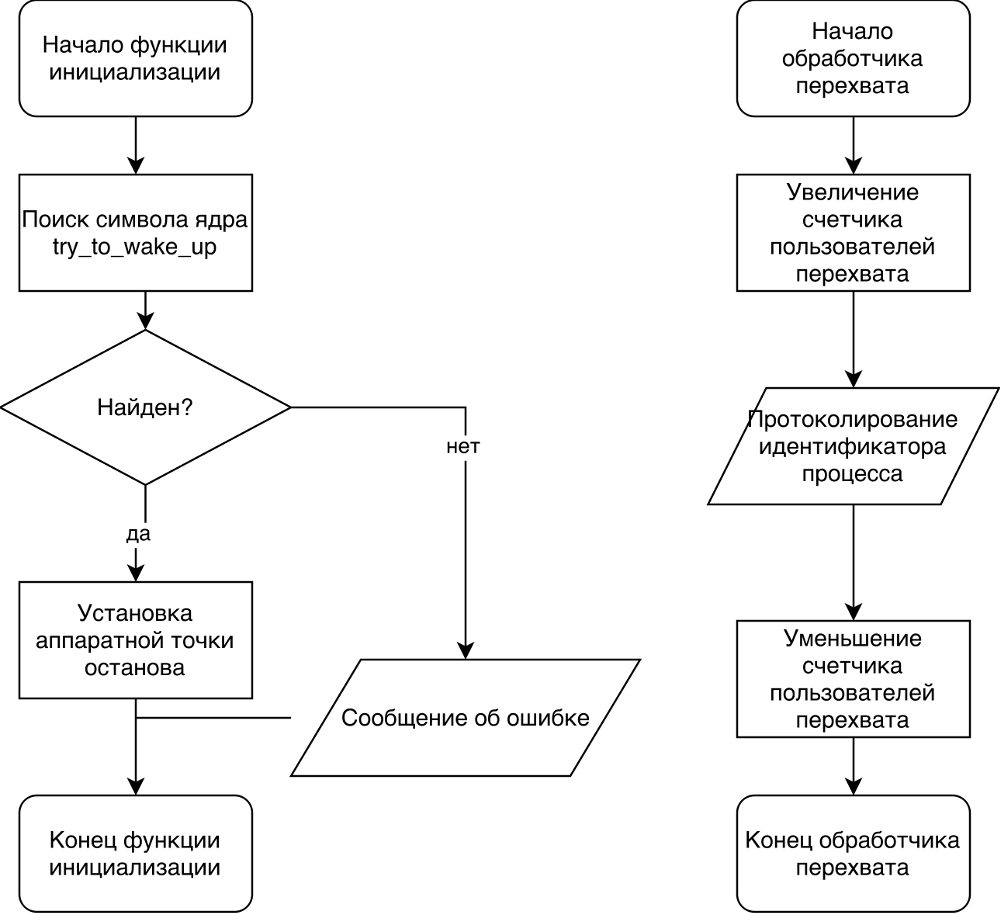
\includegraphics[height=0.4\textheight]{images/hook_scheduler.png}
\hfill
\vfill

\appsection{Алгоритм функционирования метода выявления скрытых сетевых
  соединений}{app:unhidenet}

\hfill
\vfill
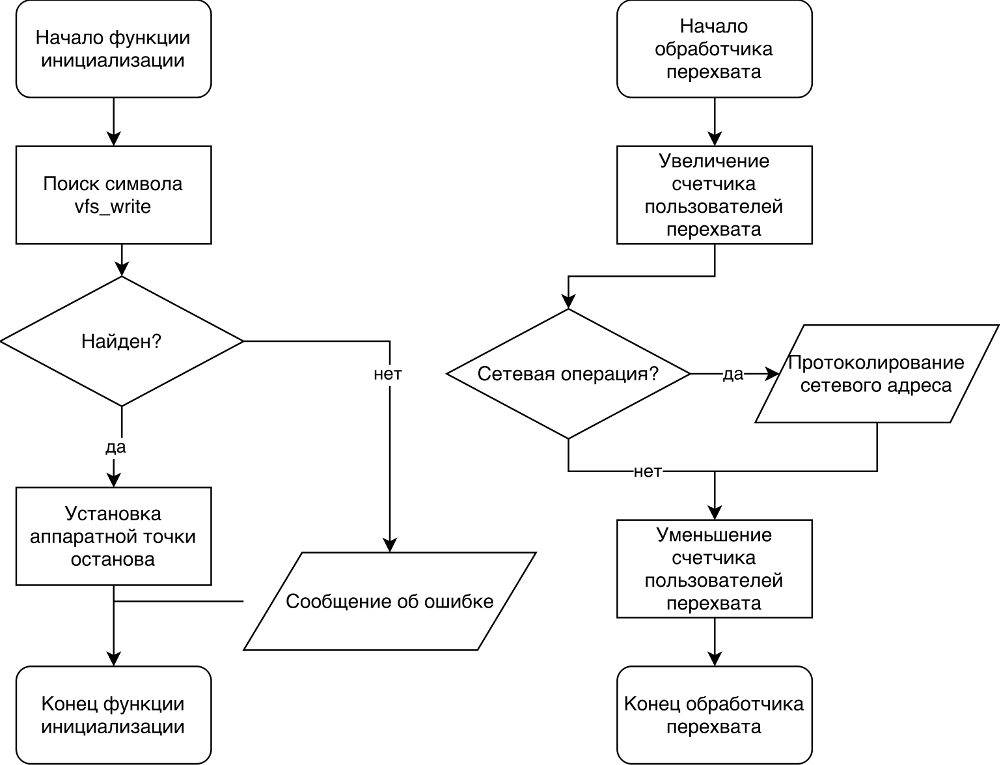
\includegraphics[height=0.4\textheight]{images/hook_net.png}
\hfill
\vfill

\appsection{Алгоритм функционирования метода выявления скрытых
  объектов файловой системы}{app:unhidefs}

\hfill
\vfill
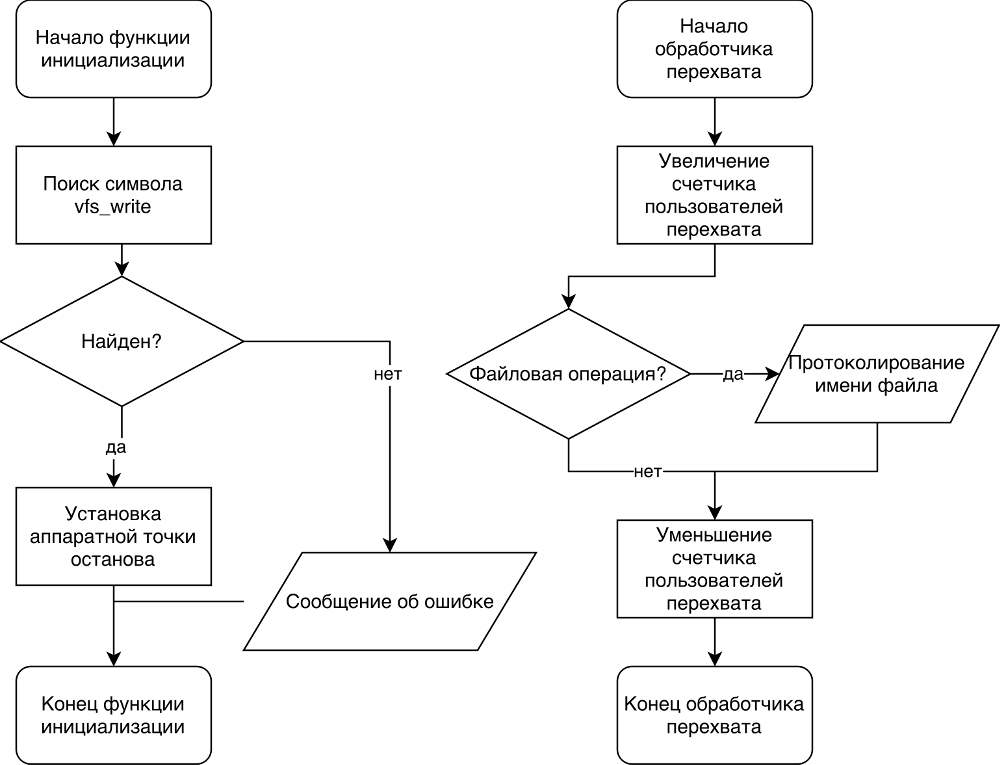
\includegraphics[height=0.4\textheight]{images/hook_fs.png}
\hfill
\vfill

\appsection{Схема планировщика задач ядра Linux}{app:scheduler}

\hfill
\vfill
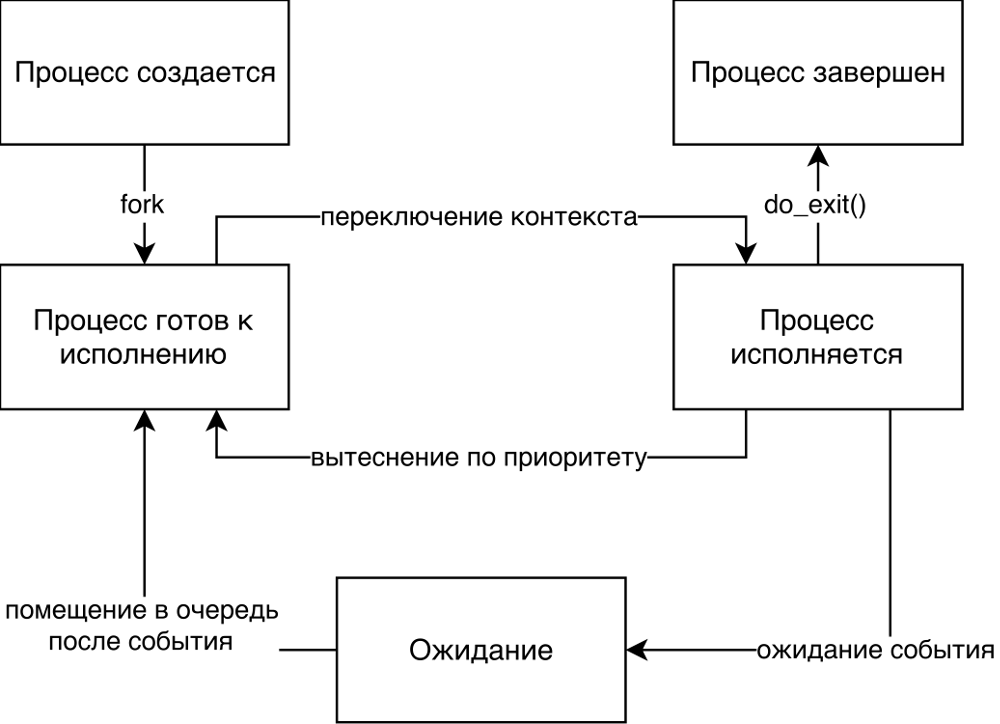
\includegraphics[height=0.4\textheight]{images/scheduler.png}
\hfill
\vfill

\appsection{Схема слоя виртуальных файловых систем ядра Linux}{app:vfs}

\hfill
\vfill
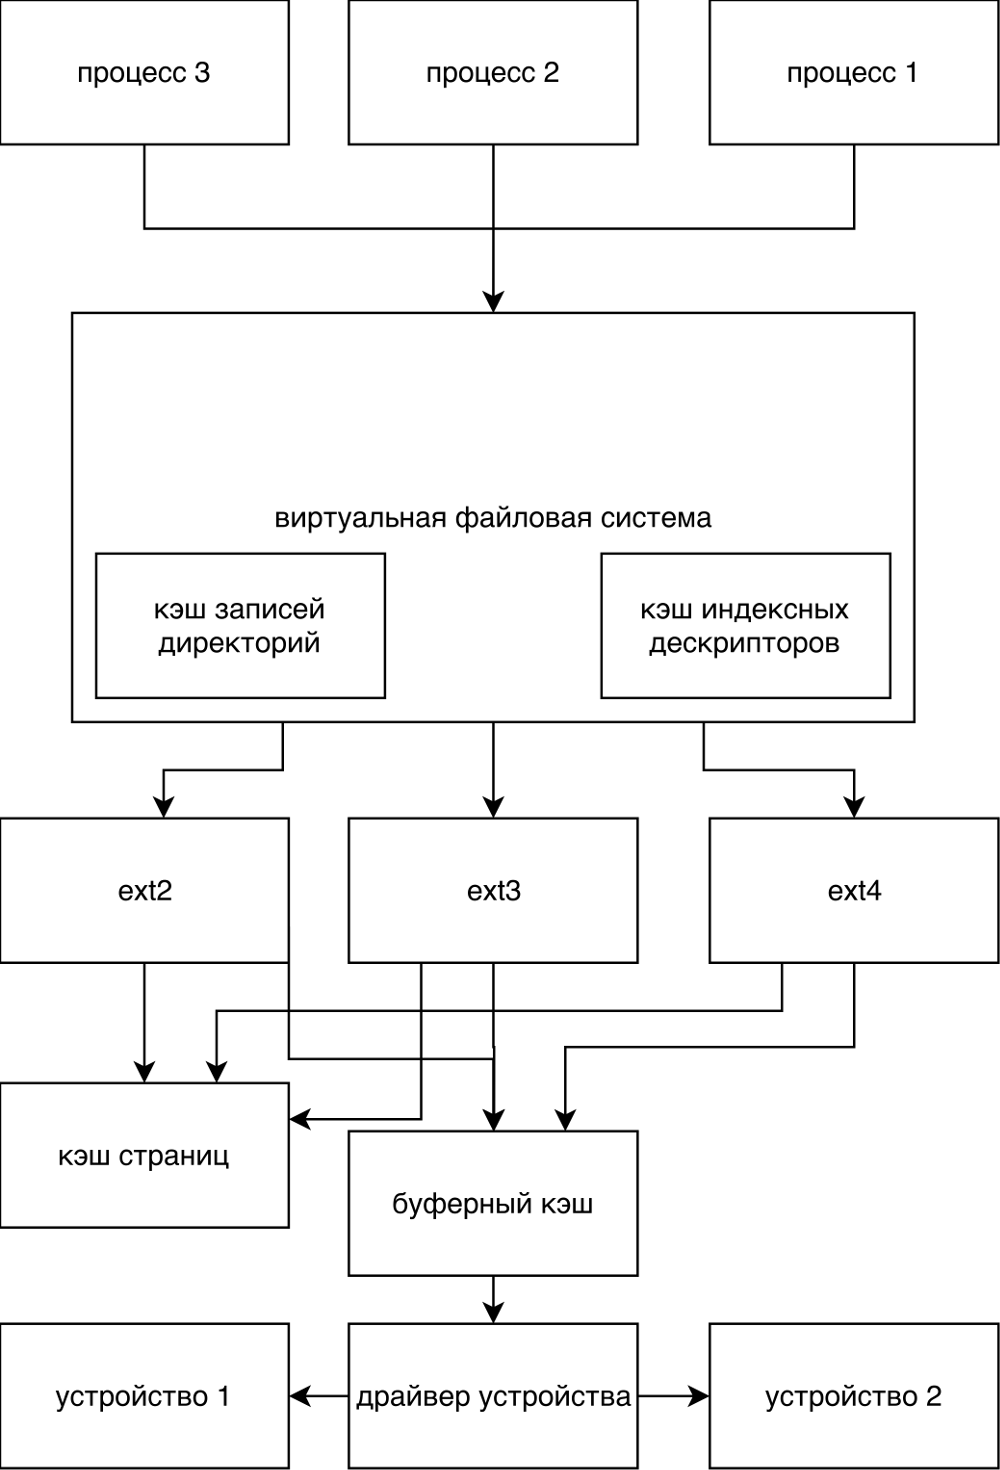
\includegraphics[width=0.8\textwidth]{images/vfsscheme.png}
\hfill
\vfill

\appsection{Схема сетевого стека ядра Linux}{app:net}

\hfill
\vfill
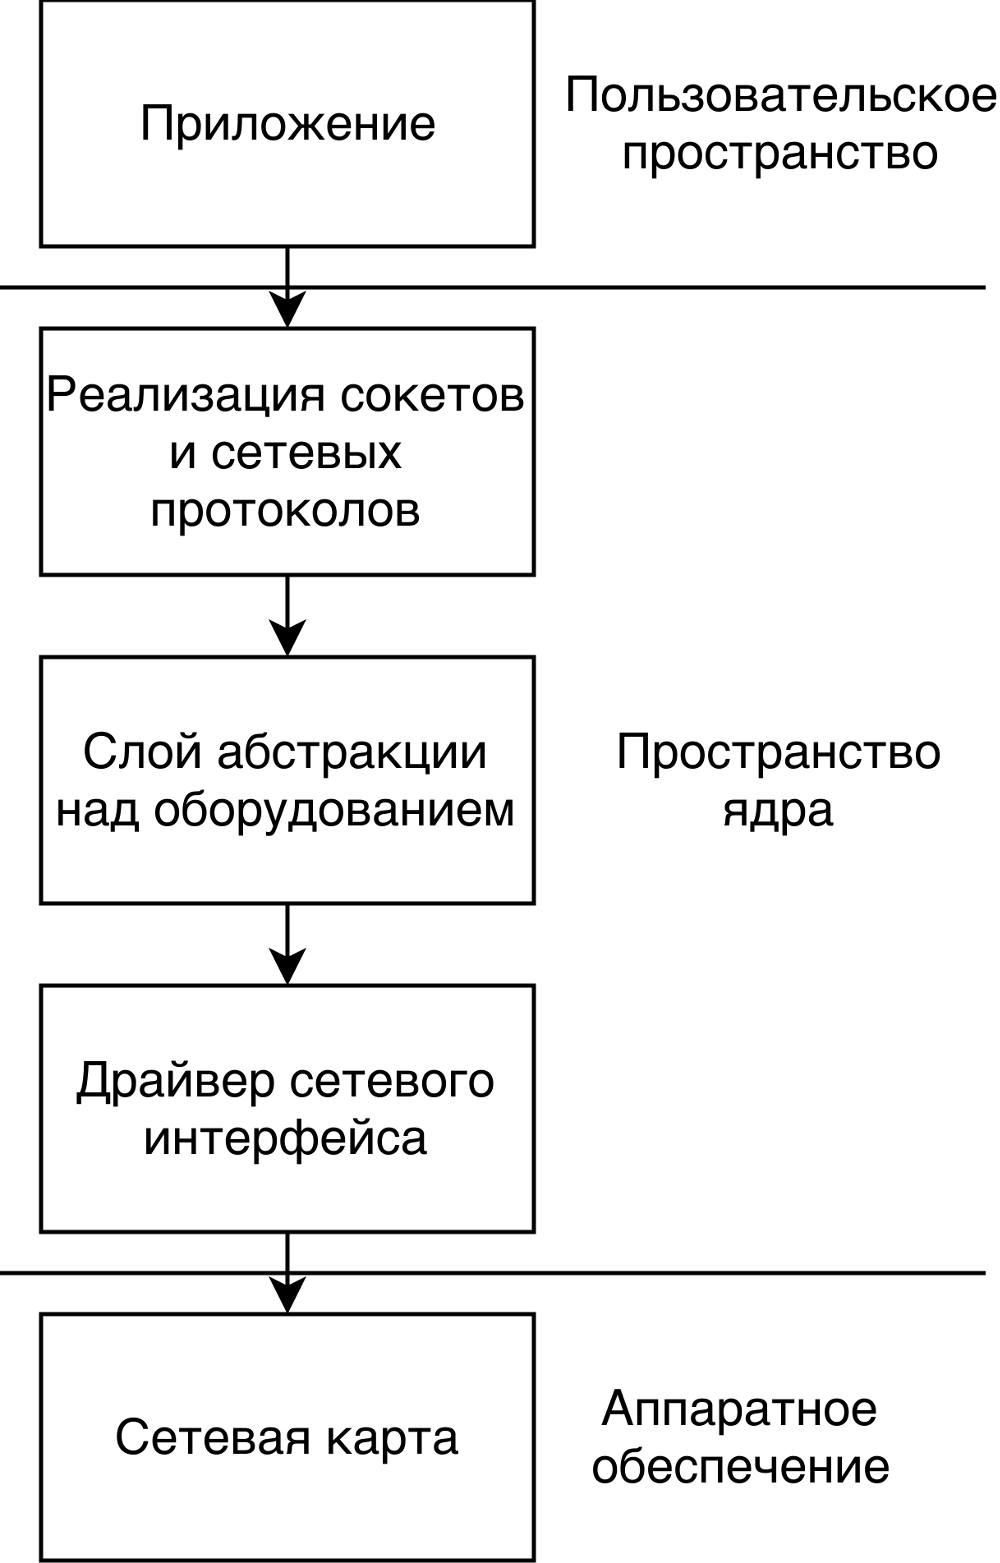
\includegraphics[width=0.6\textwidth]{images/networking.png}
\hfill
\vfill

\appsection{Акт о внедрении}{app:akt}
\begin{centering}
  
\includegraphics[height=\textheight]{signed/akt.signed.png}
\end{centering}

\end{document}
